\documentclass[xcolor=dvipsnames,10pt]{beamer}
\usepackage[english]{babel}
\usepackage[utf8]{inputenc}
\usepackage{pict2e}
\usepackage{colortbl}
\usepackage{graphicx}
\usepackage{pdfpages}
\usepackage{verbatim}
\usepackage{pgf}
%%%%%%%%%%%%%%%%%%%%
%%% nice math
\usepackage{amssymb}
\usepackage{amsmath}
\usepackage{latexsym}
\usepackage{amsthm}
\usepackage{slashed}
%%%%%%%%%%%%%%%%%%%%
%%% font type
%\usepackage{times}
\usepackage{bookman}
%\usepackage{palatino}
%\usepackage{newcent}
%\usepackage{avant}
\usefonttheme{serif}

\input{/home/antonella/Documents/Physics/mycommands.tex}

%%% nice tables
\usepackage{booktabs}
\usepackage{multirow}

\usepackage{fancybox}

%%% code pieces
\usepackage{listings}
\lstset{basicstyle=\tiny,language=c,emphstyle=\color{red},columns=fullflexible,
keepspaces=false, keywordstyle=\tiny\color{blue}, showstringspace=false} 
\newcommand\BackgroundPicture[1]{%
   \setbeamertemplate{background}{%
   \parbox[c][\paperheight]{\paperwidth}{%
       \vfill \hfill
\includegraphics[width=0.6\paperwidth,height=0.6\paperheight]{#1}
        \hfill \vfill
     }}}

%\setbeamertemplate{headline}

%%% to allow small margin
\newenvironment{changemargin}[2]{%
  \begin{list}{}{%
    \setlength{\topsep}{0pt}%
    \setlength{\leftmargin}{#1}%
    \setlength{\rightmargin}{#2}%
    \setlength{\listparindent}{\parindent}%
    \setlength{\itemindent}{\parindent}%
    \setlength{\parsep}{\parskip}%
  }%
  \item[]}{\end{list}} 

%\usetheme{Luebeck}
%\usecolortheme{seagull}
%\usecolortheme[named=BrickRed]{structure}


\usetheme[headheight=.13\textheight,footheight=.035\textheight]{boxes}
\definecolor{light-gray}{gray}{0.9}
%\definecolor{myfading}{fg=white,bg=light-gray}
\definecolor{structure2}{rgb}{1,1,1}

\mode<presentation>
%\usecolortheme[named=NavyBlue]{structure}
%\usecolortheme[named=Plum]{structure}
%\usecolortheme[named=Violet]{structure}
%\usecolortheme[named=BurntOrange]{structure}
\usecolortheme[named=RedViolet]{structure}
%\usecolortheme[named=Sepia]{structure}
\setbeamercolor{normal text}{fg=black!70!light-gray,bg=white}
\setbeamercolor{alerted text}{fg=BrickRed,bg=light-gray}
\setbeamercolor{boxcolor}{fg=black!70!light-gray,bg=structure!30!white}
\setbeamercolor{whiteboxcolor}{fg=black!70!light-gray,bg=white}

\definecolor{links}{named}{Plum}

\usepackage{hyperref}
\hypersetup{colorlinks=true,linkcolor=,urlcolor=links}

\setbeamercolor{head/foot boxes}{fg=structure!90!white,bg=structure!30!white}
\setbeamercolor{head/foot boxes bis}{fg=structure!60!white,bg=structure!90!white}

\setbeamercolor{head/foot text}{fg=structure!40!black,bg=structure!30!white}


\addheadboxtemplate{\usebeamercolor[bg]{head/foot boxes}}{\usebeamercolor[fg]{head/foot text}\logo{
\includegraphics[height=1.2cm]{pics/atlasifae2}}\raisebox{-1.8ex}{\insertlogo}
\hfill\insertshorttitle \hskip0.3cm}
\addheadboxtemplate{\usebeamercolor[fg]{head/foot boxes}}{\usebeamercolor[bg]{head/foot text}\scriptsize\hskip0.3cm\insertsectionhead}

\addfootboxtemplate{\usebeamercolor[fg]{head/foot boxes}}{\usebeamercolor[bg]{head/foot text}\hskip0.3cm\insertshortauthor\\\insertshortinstitute \hfill}
\addfootboxtemplate{\usebeamercolor[fg]{head/foot boxes bis}}{\usebeamercolor[fg]{head/foot text}\hfill\insertdate\hfill}

\def\insertpresentationendframe{\inserttotalframenumber}
\makeatletter
\g@addto@macro{\appendix}{\immediate\write\@auxout{\string\@writefile{nav}{\noexpand\headcommand{\noexpand\def\noexpand\insertpresentationendframe{\the\c@framenumber}}}}}
\makeatother

\addfootboxtemplate{\usebeamercolor[bg]{head/foot boxes}}{\usebeamercolor[fg]{head/foot text}\hfill\insertframenumber/\insertpresentationendframe\hskip0.3cm}
%\addfootboxtemplate{\usebeamercolor[bg]{head/foot boxes}}{\usebeamercolor[fg]{head/foot text}\hfill\insertframenumber/\insertpresentationendpage\hskip0.3cm}

%\setbeamertemplate{footline}{%
%  \begin{beamercolorbox}{section in head/foot}
%\begin{center}
%\begin{tabular}{lcr}
%\hskip45pt \textit{Barcelona plans for u4u4 searches in lepton+jets} \phantom{a/aa} & 2011, December 21st \phantom{a/aa} \insertframenumber / %\insertpresentationendpage
%\\
%\end{tabular}
%\end{center}  \end{beamercolorbox}
%}


%\usesectionheadtemplate
%{\color{white}\tiny\textbf{\insertsectionhead}}
%{\color{structureshaded}\tiny\textbf{\insertsectionhead}}


%\useoutertheme{sidebar}
%\setbeamertemplate{sidebar canvas left}[vertical shading][top=White,bottom=Gray]
%\setbeamertemplate{sidebar canvas left}[vertical shading][top=White,bottom=CadetBlue]
%\setbeamertemplate{sidebar canvas left}[vertical shading][top=White,bottom=YellowGreen]
%\setbeamertemplate{sidebar canvas left}[vertical shading][top=White,bottom=light-gray]

\setbeamertemplate{navigation symbols}{}
\setbeamersize{text margin left=.2cm,text margin right=.2cm} 






\AtBeginSection[]
{
  \begin{frame}\centering
    \frametitle{Outline}
    \tableofcontents[currentsection]
  \end{frame}
}



\title[]{Searches for vector-like quarks\\ with the ATLAS detector}
\author[A Succurro]{Antonella Succurro\\ \vspace{\baselineskip}\textit{\small on behalf of}\\ the ATLAS collaboration}
\institute[\, \emph{IFAE Barcelona}]{}
\date{EPS 2013, Stockholm, July 18th-24th}


\begin{document}

\frame{

\vspace{-.8cm}


\maketitle\centering

\vspace{-.8cm}

}

%\begin{frame}\frametitle{Content}
%\end{frame}
%\begin{frame}\frametitle{Outline}
%\centering
%\tableofcontents[part=1,pausesections]
%\tableofcontents
%\end{frame}

%----------------------------------
\section{Introduction}
%----------------------------------

\begin{frame}\frametitle{Standard Model as an effective theory}
\scriptsize\centering

\myskip

%The Standard Model works well at low energies, but what about \alert{higher energies}, like the ones accessible now at the LHC?\\
The Standard Model does not provide answers to the following questions
\myskip
\begin{itemize}
\item Where does the baryon asymmetry come from?
\item What is Dark Matter?
\item How to solve the hierarchy problem?
\end{itemize}

\begin{flushright}\it Supersymmetry is not the only possible solution\dots\end{flushright}


Extra-dimensions~\cite{Csaki:2004ay}, composite Higgs~\cite{Perelstein:2005ka} models\\
with \alert{new heavy quarks predicted}~\cite{AguilarSaavedra:2009es}

\myskip

\begin{minipage}{.5\textwidth}

\begin{itemize}
\item Not chiral$^{(a)}$: chiral 4th generation would change the Higgs SM cross section and B.R.
\item Vector-like: left and right components transform the same under $SU(2)\times U(1)$
\item Weak-isospin singlets, doublets or triplets
\end{itemize}

\begin{flushright}\it naturally solve the  hierarchy problem,$\;\;$\\
like a stop squark in SUSY$\;\;$ \end{flushright}

\tiny
$^{(a)}$ still, some models allow for a chiral fourth generation, see e.g.~\cite{Cetin:2011aa}
\end{minipage}\begin{minipage}{.5\textwidth}\centering

{\tiny
\begin{tabular}{|lc|lc|}\toprule\hline
&&&\\
\scriptsize\multirow{2}{*}{Singlet} & \scriptsize Decay & \scriptsize\multirow{2}{*}{Doublets} &\scriptsize Decay \\ 
\scriptsize& \scriptsize modes & &\scriptsize modes\\
& & &\\
$T(+2/3)$ & $W^+b,\, Ht,\, Zt$ & \multirow{2}{*}{$\bigg(\begin{array}{c}T \\ B\end{array}\bigg)$} & $W^+b,\, Ht,\, Zt$\\ 
& & & $ W^-t,\, Hb,\, Zb$\\
$B(-1/3)$ & $ W^-t,\, Hb,\, Zb$ & & \\
& & \multirow{2}{*}{$\bigg(\begin{array}{c}T \\ X\end{array}\bigg)$} & $Ht,\, Zt$\\
$X(+5/3)$ & $W^+t$ & & $W^+t$\\
& & &\\
$Y(-4/3)$ & $W^-b$ & \multirow{2}{*}{$\bigg(\begin{array}{c}B \\ Y\end{array}\bigg)$} & $Hb,\, Zb$\\
& & & $W^-b$\\
&&&\\\hline\bottomrule
\end{tabular}
}
\end{minipage}


\end{frame}




\begin{frame}\frametitle{Heavy quark production}
\scriptsize\centering


\myskip

\begin{minipage}{.8\textwidth}
\begin{pgfpicture}{0.0\textwidth}{0.0\textheight}{1.\textwidth}{.6\textwidth}
\pgfdeclareimage[interpolate=true,width=.78\textwidth]{xsec}{pics/xsecJA}%ztag/fig_01b}
\pgfputat{\pgfxy(-1.5,0)}{\pgfbox[left,base]{\pgfuseimage{xsec}}}
\pgfdeclareimage[interpolate=true,width=.45\textwidth]{feynd}{feynQQ}%{ztag/fig_01a}
\pgfputat{\pgfxy(6.2,3.3)}{\pgfbox[left,base]{\pgfuseimage{feynd}}}

{\usebeamercolor[fg]{head/foot boxes}
\pgfputat{\pgfxy(2.2,5.)}{\pgfbox[left,center]{\normalsize from~\cite{Aguilar-Saavedra:2013qpa}}}
}

\pgfputat{\pgfxy(6.2,3.)}{\pgfbox[left,center]{Pair-production via \alert{strong interaction}}}
%\colorlet{}
      \only<2>{
    \begin{pgftranslate}{\pgfpoint{-0.4\textwidth}{0.15\textheight}}
{\usebeamercolor[fg]{head/foot boxes}
%\pgfrect[fill]{\pgfxy(5.5,3.45)}{\pgfxy(2,0.1)}
%\pgfrect[fill]{\pgfxy(5.5,1)}{\pgfxy(0.1,4)}
\begin{pgfscope}
\pgfsetlinewidth{1.5pt}
\pgfmoveto{\pgfxy(5.4,2.2)}
\pgfcurveto{\pgfxy(4.3,-3)}{\pgfxy(7.3,2)}{\pgfxy(5.6,2.8)}
\pgfstroke
\pgfmoveto{\pgfxy(5.4,2.2)}
\pgfcurveto{\pgfxy(5.5,2.5)}{\pgfxy(5.6,2.7)}{\pgfxy(5.8,2.4)}
\pgfstroke
{\pgfsetendarrow{\pgfarrowlargepointed{6pt}}
\pgfline{\pgfxy(5.8,1)}{\pgfxy(10.3,0.2)}}
\end{pgfscope}
}
    \end{pgftranslate}
\pgfputat{\pgfxy(6.9,1.3)}{\pgfbox[left,center]{\alert{EW single production}}}
\pgfputat{\pgfxy(6.5,1.0)}{\pgfbox[left,center]{could dominate at high mass}}
      }
\end{pgfpicture}
\end{minipage}

\end{frame}



\section{General Strategy}


\begin{frame}\frametitle{Heavy quark decay modes}
\scriptsize\centering
\myskip

B.R.s are very model dependent

\begin{itemize}
\item most analyses optimized for specific decay channels
\end{itemize}


\begin{pgfpicture}{0.0\textwidth}{0.0\textheight}{1.\textwidth}{.6\textwidth}

\pgfdeclareimage[interpolate=true,width=.5\textwidth]{brVLT}{ztag/fig_02a}
\pgfputat{\pgfpoint{0.0\textwidth}{0.15\textheight}}{\pgfbox[left,base]{\pgfuseimage{brVLT}}}

\pgfdeclareimage[interpolate=true,width=.5\textwidth]{brVLB}{ztag/fig_02b}
\pgfputat{\pgfpoint{0.5\textwidth}{0.15\textheight}}{\pgfbox[left,base]{\pgfuseimage{brVLB}}}

%\colorlet{}
{\usebeamercolor[bg]{head/foot boxes}
%\pgfrect[fill]{\pgfxy(5.5,3.45)}{\pgfxy(2,0.1)}
%\pgfrect[fill]{\pgfxy(5.5,1)}{\pgfxy(0.1,4)}
\begin{pgfscope}
\pgfsetlinewidth{1.5pt}
%\pgfmoveto{\pgfpoint{0.25\textwidth}{0.25\textheight}}
%\pgfline{\pgfpoint{0.25\textwidth}{0.65\textheight}}{\pgfpoint{0.5\textwidth}{0.65\textheight}}
    \begin{pgftranslate}{\pgfpoint{0.35\textwidth}{0.65\textheight}}
{\usebeamercolor[fg]{head/foot boxes}
\pgfputat{\pgfxy(-1.,1.75)}{\pgfbox[left,base]{\textbf{\large $T$}}}
\pgfputat{\pgfxy(5.2,1.75)}{\pgfbox[left,base]{\textbf{\large $B$}}}
}
    \end{pgftranslate}
      \only<2>{
    \begin{pgftranslate}{\pgfpoint{0.35\textwidth}{0.65\textheight}}
\pgfzeroellipse{\pgfxy(1.6,0)}{\pgfxy(0,0.15)}
\pgfstroke
\pgfputat{\pgfxy(-2.2,0)}{\pgfbox[left,base]{\textbf{\large\#1}}}
    \end{pgftranslate}
      }
      \only<3>{
    \begin{pgftranslate}{\pgfpoint{0.78\textwidth}{0.7\textheight}}
\pgfzeroellipse{\pgfxy(2.3,0)}{\pgfxy(0,0.8)}
\pgfstroke
\pgfputat{\pgfxy(1.2,-0.4)}{\pgfbox[left,base]{\textbf{\large\#2}}}
    \end{pgftranslate}
      }
      \only<4>{
    \begin{pgftranslate}{\pgfpoint{0.535\textwidth}{0.686\textheight}}
\pgfzeroellipse{\pgfxy(4,0)}{\pgfxy(0,0.18)}
\pgfstroke
\pgfputat{\pgfxy(-4.5,0.2)}{\pgfbox[left,base]{\textbf{\large\#3}}}
    \end{pgftranslate}
      }
      \only<5>{
    \begin{pgftranslate}{\pgfpoint{0.35\textwidth}{0.725\textheight}}
\pgfzeroellipse{\pgfxy(1.6,0)}{\pgfxy(0,0.15)}
\pgfstroke
\pgfputat{\pgfxy(-2.2,0)}{\pgfbox[left,base]{\textbf{\large\#4}}}
    \end{pgftranslate}
      }
\end{pgfscope}
}
\end{pgfpicture}


\end{frame}




\begin{frame}\frametitle{Model Independent Strategy $\;$\small \dots since Oct 2012~\cite{ATLAS:2012qe}!}
\footnotesize\centering


\begin{pgfpicture}{0.0\textwidth}{0.0\textheight}{1.\textwidth}{.6\textwidth}

\begin{pgfscope}
\onslide<1->{
    \pgfsetendarrow{\pgfarrowlargepointed{6pt}}
    \pgfsetlinewidth{1.5pt}
    \usebeamercolor[fg]{head/foot boxes}
    \begin{pgftranslate}{\pgfpoint{0.1\textwidth}{0.15\textheight}}
\pgfline{\pgfxy(0,0)}{\pgfxy(5.5,0)}
\pgfstroke
\pgfputat{\pgfxy(3.5,-0.5)}{\pgfbox[left,base]{BR($T\to Wb$)}}
    \usebeamercolor[bg]{head/foot boxes}
\pgfputat{\pgfxy(3.5,-0.8)}{\pgfbox[left,base]{BR($B\to Wt$)}}
    \usebeamercolor[fg]{normal text}
\pgfcircle[fill]{\pgfxy(6.8,4.1)}{2pt}
\pgfputat{\pgfxy(7,4)}{\pgfbox[left,base]{Build a 2-dim plane}}
\pgfputat{\pgfxy(7,3.7)}{\pgfbox[left,base]{to scan model mixing}}
%    \end{pgftranslate}
%\end{pgfscope}
}
%\pause
\onslide<2->{
%\begin{pgfscope}
    \pgfsetendarrow{\pgfarrowlargepointed{6pt}}
    \pgfsetlinewidth{1.5pt}
    \usebeamercolor[fg]{head/foot boxes}
%    \begin{pgftranslate}{\pgfpoint{0.1\textwidth}{0.15\textheight}}
    \usebeamercolor[fg]{head/foot boxes}
\pgfline{\pgfxy(0,0)}{\pgfxy(0,5.5)}
\pgfstroke
    \begin{pgfrotateby}{\pgfdegree{90}}
\pgfputat{\pgfxy(3.5,0.4)}{\pgfbox[left,base]{BR($T\to Ht$)}}
    \usebeamercolor[bg]{head/foot boxes}
\pgfputat{\pgfxy(3.5,0.7)}{\pgfbox[left,base]{BR($B\to Hb$)}}
    \end{pgfrotateby}
%    \end{pgftranslate}
%\end{pgfscope}
}
%\pause
\onslide<3->{
%\begin{pgfscope}
    \pgfsetlinewidth{1.5pt}
    \color{light-gray}
%    \begin{pgftranslate}{\pgfpoint{0.1\textwidth}{0.15\textheight}}
%\pgfline{\pgfxy(5,0)}{\pgfxy(0,5)}
%\pgfstroke
\pgfmoveto{\pgfxy(5,0)}
\pgflineto{\pgfxy(5,5)}
\pgflineto{\pgfxy(0,5)}
%\pgfstroke
\pgffill
    \color{gray}
\pgfputlabelrotated{0.5}{\pgfxy(0,5)}{\pgfxy(5,0)}{8pt}{\pgfbox[center,base]{Forbidden}}
    \usebeamercolor[fg]{normal text}
\pgfcircle[fill]{\pgfxy(6.8,3.3)}{2pt}
\pgfputat{\pgfxy(7,3.2)}{\pgfbox[left,base]{Sum of BRs is 1$^{(a)}$}}
%\pgfputat{\pgfxy(5.2,0.7)}{\pgfbox[left,base]{\scriptsize $^{(a)}$BR($T\to  Zt/b$) = 1 - BR($T\to Ht/b$) - BR($T\to Wb/t$)}}
\pgfputat{\pgfxy(5.9,-0.4)}{\pgfbox[left,base]{\scriptsize $^{(a)}$BR($T/B\to  Zt/b$) = 1 - BR($T/B\to Ht/b$) }}
\pgfputat{\pgfxy(8.755,-0.7)}{\pgfbox[left,base]{\scriptsize - BR($T/B\to Wb/t$)}}

%    \end{pgftranslate}
%\end{pgfscope}
}
%\pause
\onslide<4->{
%\begin{pgfscope}
    \pgfsetlinewidth{1.5pt}
%    \begin{pgftranslate}{\pgfpoint{0.1\textwidth}{0.15\textheight}}
    \usebeamercolor[fg]{normal text}
\pgfcircle[fill]{\pgfxy(6.8,2.8)}{2pt}
\pgfputat{\pgfxy(7,2.7)}{\pgfbox[left,base]{Different analyses are}}
\pgfputat{\pgfxy(7,2.4)}{\pgfbox[left,base]{sensitive to different areas}}
    \usebeamercolor[fg]{head/foot boxes}
\begin{pgfscope}
\pgfmoveto{\pgfxy(5,0)}
\pgflineto{\pgfxy(0,0)}
\pgflineto{\pgfxy(0,5)}
\pgfclip
\pgfcircle[fill]{\pgfxy(.5,4)}{35pt}
{\usebeamercolor[bg]{normal text}
%\pgfputat{\pgfxy(0.,3.5)}{\begin{pgfrotateby}{\pgfdegree{-45}}\pgfbox[left,base]{$T(B)\to Ht(b)$}\end{pgfrotateby}}
\pgfputat{\pgfxy(0.,3.6)}{\pgfbox[left,base]{\large$Ht(b)$}}
}
}
\onslide<5->{
%\pause
\pgfcircle[fill]{\pgfxy(.6,.6)}{35pt}
{\usebeamercolor[bg]{normal text}
%\pgfputat{\pgfxy(0.2,.4)}{\pgfbox[left,base]{$T(B)\to Zt(b)$}}
\pgfputat{\pgfxy(0.2,.4)}{\pgfbox[left,base]{\large$Zt(b)$}}
}
}
\onslide<6->{
%\pause
\pgfcircle[fill]{\pgfxy(4,0)}{35pt}
{\usebeamercolor[bg]{normal text}
%\pgfputat{\pgfxy(3.,0.4)}{\pgfbox[left,base]{$T(B)\to Wb(t)$}}
\pgfputat{\pgfxy(3.2,0.4)}{\pgfbox[left,base]{\large$Wb(t)$}}
}
}
\end{pgfscope}
\onslide<7->{
\pgfcircle[fill]{\pgfxy(6.8,2.)}{2pt}
\pgfputat{\pgfxy(7,1.9)}{\pgfbox[left,base]{Set exclusion using}}
\pgfputat{\pgfxy(7,1.6)}{\pgfbox[left,base]{$CL_{s}$ technique~\cite{Junk:1999kv,Read:2002hq}}}
\pgfcircle[fill]{\pgfxy(6.8,1.2)}{2pt}
{\usebeamercolor[fg]{normal text}
\pgfputat{\pgfxy(7,1.1)}{\pgfbox[left,base]{Using \alert{14.3\ifb}\ of 2012 data}}}
}

\onslide<8->{
\pgfdeclareimage[interpolate=true,width=.45\textwidth]{wbwb7tev}{pics/wbwb7tev}
\pgfputat{\pgfxy(0.0,0.0)}{\pgfbox[left,base]{\pgfuseimage{wbwb7tev}}}
\pgfcircle[fill]{\pgfxy(6.8,0.7)}{2pt}
{\usebeamercolor[fg]{normal text}
\pgfputat{\pgfxy(7,0.6)}{\pgfbox[left,base]{Updating 7~TeV results}}
}
}
    \end{pgftranslate}
\end{pgfscope}
\end{pgfpicture}

\end{frame}



%%%%%%%%%%%%%%%%%%%%%%%%%%%%%%
\section{$T\bar{T}\to Ht+X$}
%%%%%%%%%%%%%%%%%%%%%%%%%%%%%%

\begin{frame}\frametitle{$T\bar{T}\to Ht+X\qquad\qquad$\small ATLAS-CONF-2013-018~\cite{ATLAS-CONF-2013-018}}
\footnotesize\centering

Channel with high jet and $b$-tagged jet multiplicity ($H\to bb$, $t\to Wb$)

%\myskip
  \begin{minipage}{.55\textwidth}\scriptsize\centering

       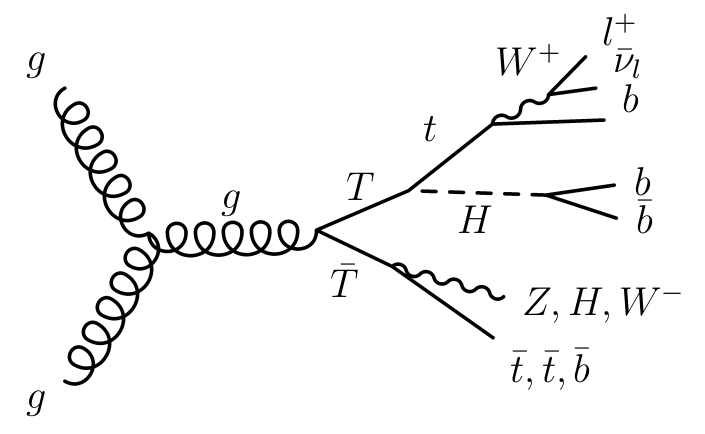
\includegraphics[width=.5\textwidth]{htx/feynhtx}

  \begin{minipage}{.4\textwidth}\tiny\centering

       \begin{itemize}
\item At least 6 jets with $p_T>25~$GeV
\item Exactly one well reconstructed, isolated lepton ($e$ or $\mu$)
\item ${E}^{\rm miss}_T >$20~GeV
\item ${E}^{\rm miss}_T + m_T(W)>$60~GeV
       \end{itemize}

\end{minipage}\begin{minipage}{.6\textwidth}\centering

\myskip

\alert{Discriminant variable}: \\$H_T=\sum_j p_T(j) + p_T(l) + {E}^{\rm miss}_T$

       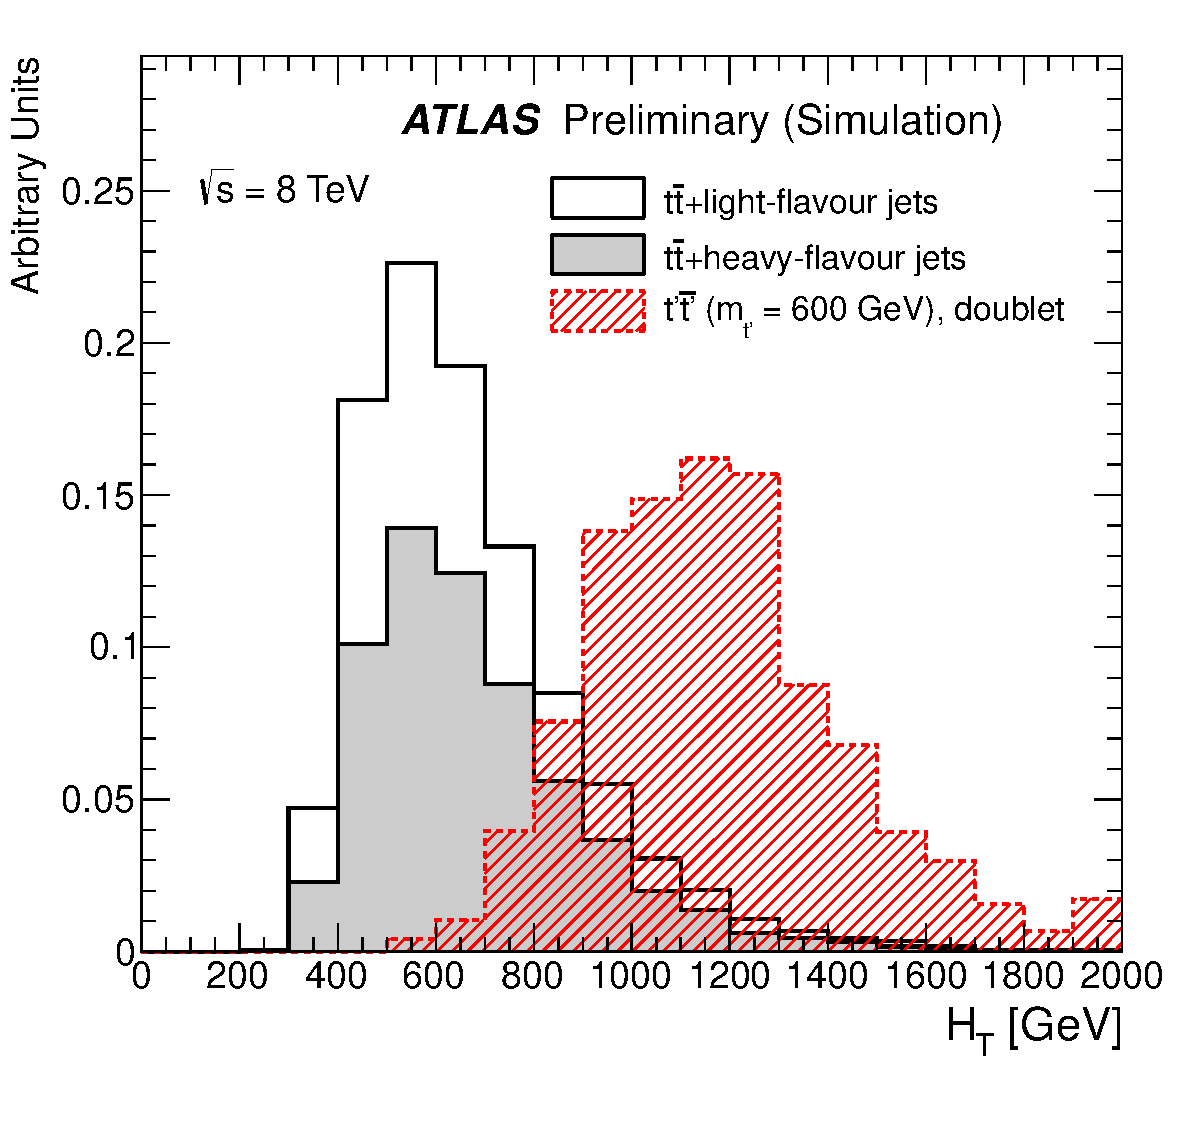
\includegraphics[width=1.\textwidth]{htx/fig_02b.pdf}


\end{minipage}

     \end{minipage}\begin{minipage}{.45\textwidth}\centering


\begin{minipage}{1.\textwidth}\centering

\myskip

       Three channels:\\ $=2$, $=3$, \alert{$\geq 4$ $b$-tagged jets}

       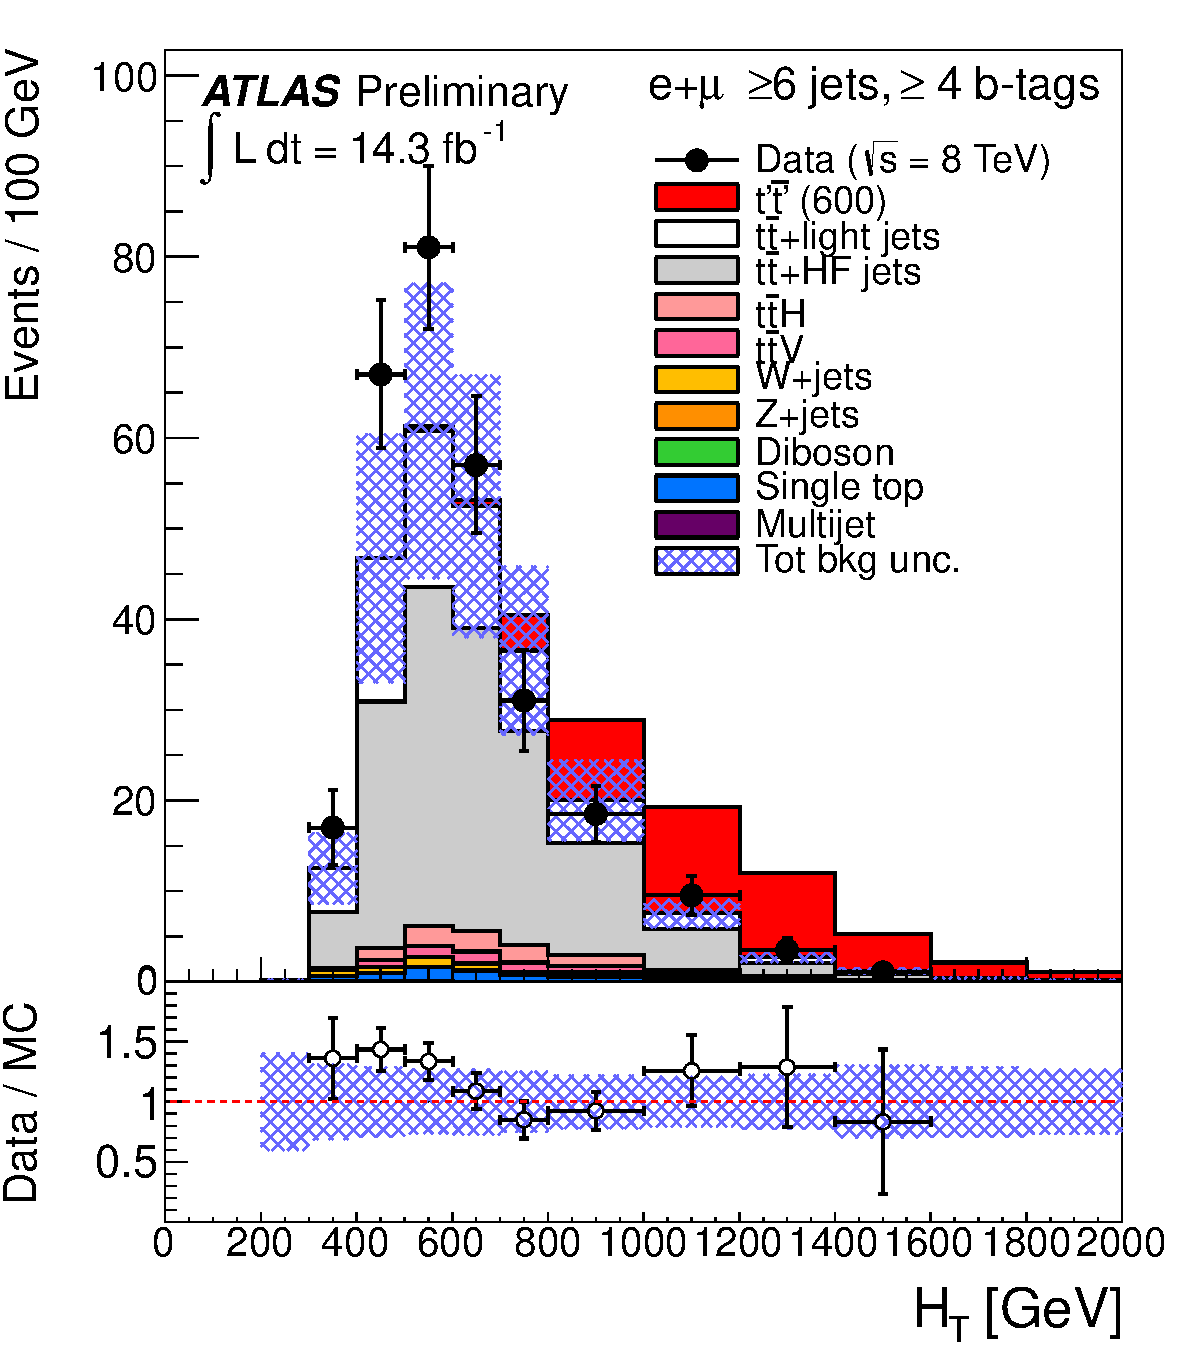
\includegraphics[width=.8\textwidth]{htx/fig_04c.pdf}

\begin{flushright}
\vskip-3ex
\textit{\scriptsize N$_{\rm tag}=2,3$ help constrain\\ background systematics}
\end{flushright}
     \end{minipage}
\end{minipage}

\end{frame}



\begin{frame}\frametitle{$T$ exclusion plane~\cite{combination} I}
\footnotesize\centering

\includegraphics[width=1.\textwidth]{comb2d/ATLAS_VLQ_TT_june2013_step1}

\end{frame}


%%%%%%%%%%%%%%%%%%%%%%%%%%%%%%
\section{Same-sign dileptons}
%%%%%%%%%%%%%%%%%%%%%%%%%%%%%%
\begin{frame}\frametitle{Same-sign dileptons$\qquad$\small ATLAS-CONF-2013-051~\cite{ATLAS-CONF-2013-051}$\;$\tiny update of~\cite{ATLAS-CONF-2012-130}}
\footnotesize\centering

Channel with very small contamination from SM backgrounds: sensitive to many possible new physics signals like vector-like $B$ and $T$, $t\bar{t}t\bar{t}$, $\tilde{g}$

\scriptsize
\begin{minipage}{.32\textwidth}\centering
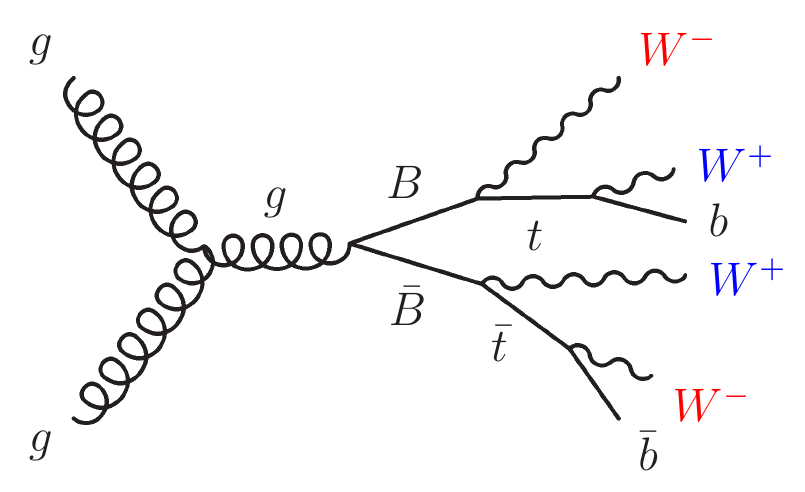
\includegraphics[width=1.\textwidth]{ssign/feynss}
  \end{minipage}\begin{minipage}{.24\textwidth}
       \begin{itemize}
       \item Exactly 2 leptons ($e$ or $\mu$) with same electric charge
       \item $Z$ veto in $ee$ and $\mu\mu$ channels
       \end{itemize}
     \end{minipage}\begin{minipage}{.22\textwidth}
       \begin{itemize}
       \item $\geq 2$ jets with $p_T>25$~GeV
       \item $\geq 1$ $b$-tagged jet 
       \end{itemize} 
     \end{minipage}\begin{minipage}{.22\textwidth}
       \begin{itemize}
       \item ${E}^{\rm miss}_T > 40~$GeV
       \item $H_T^{(1)}> 650~$GeV
       \end{itemize} 
  \end{minipage}
         \begin{table}[p]\tiny%\footnotesize
  \begin{center}
    %\caption{Observed and expected number of events  with statistical  (first) and systematic (second) uncertainties for
    %the $b^{\prime}$/VLQ signal selection.}\label{finalyieldbprime}
\begin{tabular}{l|c|c|c}
     \hline
     \hline
     Backgrounds & \multicolumn{3}{c}{Channel} \\
     \hline
     Samples & $ee$      & $e\mu$  & $\mu\mu$           \\
     \hline
     Charge misidentification    & $0.6 \pm 0.1 \pm 0.2$ & $0.9 \pm 0.1 \pm 0.3 $   & ---     \\
     Fakes    & $0.8 \pm 0.4 \pm 0.3 $ & $0.2 \pm 0.4 \pm 0.1$   & $< 1.1$     \\
     \hline
      Diboson & & & \\
      $\bullet$ $WZ/ZZ$+jets & $0.3 \pm 0.2 \pm 0.1  $ & $0.3 \pm 0.1^{+0.4}_{-0.2}$ & $0.4 \pm 0.2 \pm 0.1$\\
      $\bullet$ $W^{\pm}W^\pm$+2 jets & $0.17 \pm 0.09 \pm 0.05$ & $0.3 \pm 0.2 \pm 0.1 $ & $0.2 \pm 0.1 \pm 0.1$ \\
      \hline
      $t\bar{t}+W/Z$ & & & \\
      $\bullet$ $t\bar{t}W$(+jet(s)) & $0.6 \pm 0.2 \pm 0.3$ & $1.9 \pm 0.2 \pm 0.6$ & $1.3 \pm 0.2 \pm 0.4$\\
      $\bullet$ $t\bar{t}Z$(+jet(s)) & $0.18 \pm 0.03 \pm 0.06$ & $0.66 \pm 0.05\pm 0.22$ & $0.31 \pm 0.04 \pm 0.10$\\
      $\bullet$ $t\bar{t}W^+W^-$ & $0.024 \pm 0.003^{+0.010}_{-0.007}$ & $0.072 \pm 0.005^{+0.028}_{-0.020}$ & $0.055 \pm 0.004^{+0.022}_{-0.016}$\\
\hline
Total expected background& $2.7 \pm 0.5 \pm 0.4 $ & $4.4 \pm 0.5^{+0.9}_{-0.7}$ & $2.3 \pm 1.2 \pm 0.5$ \\
\hline
Observed & 3 & 10 & 2 \\
\hline
    \end{tabular}
  \end{center}
\end{table}




\tiny
\begin{flushright}
$(1)\ \ H_T=\sum_j p_T(j) + p_T(l_1) + p_T(l_2)$
\end{flushright}

\end{frame}



\begin{frame}\frametitle{$T$ exclusion plane~\cite{combination} II}
\footnotesize\centering

\includegraphics[width=1.\textwidth]{comb2d/ATLAS_VLQ_TT_june2013_step2}

\end{frame}


\begin{frame}\frametitle{$B$ exclusion plane~\cite{combination} I}
\footnotesize\centering

\includegraphics[width=1.\textwidth]{comb2d/ATLAS_VLQ_BB_june2013_step1}

\end{frame}




%%%%%%%%%%%%%%%%%%%%%%%%%%%%%%
\section{$B\bar{B}(T\bar{T})\to Zb(t)+X$}
%%%%%%%%%%%%%%%%%%%%%%%%%%%%%%
\begin{frame}\frametitle{$B\bar{B}(T\bar{T})\to Zb(t)+X\qquad$\small ATLAS-CONF-2013-056~\cite{ATLAS-CONF-2013-056} \tiny $\;$ update of~\cite{:2012aka}}
\footnotesize\centering

Exploit ability to reconstruct $Z$ bosons from OS dileptons ($e$ and $\mu$)


\myskip
\begin{minipage}{.6\textwidth}
\centering

\begin{minipage}{.45\textwidth}

\scriptsize
\centering

\begin{itemize}
\item Exactly two same flavor, opposite charge leptons
\item Dilepton mass in a 15~GeV mass window around $m(Z)$
\item At least two $b-$tagged jets
\end{itemize}

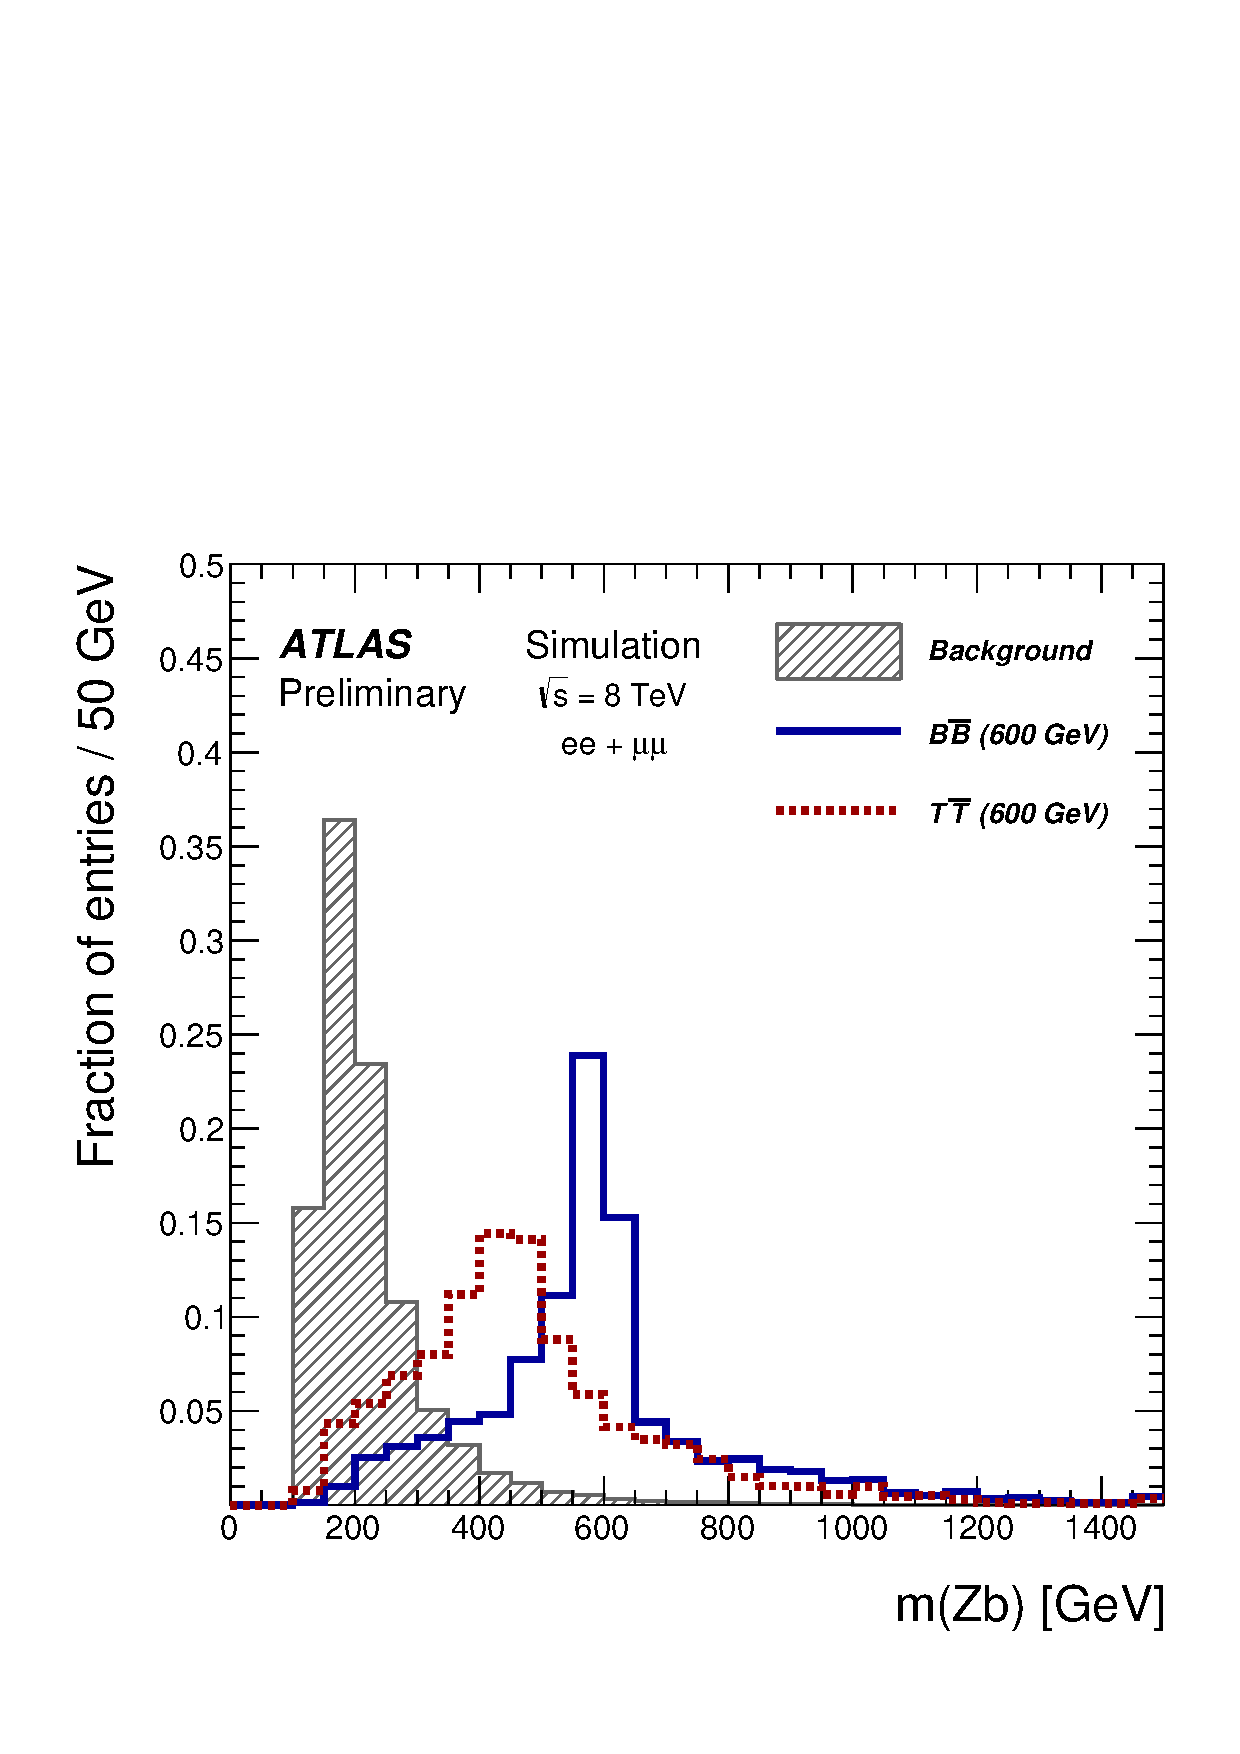
\includegraphics[width=1.1\textwidth]{ztag/fig_03d}
\end{minipage}\begin{minipage}{.55\textwidth}\centering

\begin{pgfpicture}{0.0\textwidth}{0.0\textheight}{1.\textwidth}{.6\textwidth}
   \begin{pgftranslate}{\pgfpoint{0.1\textwidth}{-0.05\textheight}}
\pgfdeclareimage[interpolate=true,width=.85\textwidth]{ntag}{ztag/fig_03a}
\pgfputat{\pgfxy(0.0,0.0)}{\pgfbox[left,base]{\pgfuseimage{ntag}}}
 \pgfsetlinewidth{1.pt}
 \usebeamercolor[bg]{head/foot boxes}
 \pgfline{\pgfxy(1.115,0.4)}{\pgfxy(1.115,2.2)}
 \pgfstroke
 \usebeamercolor[fg]{head/foot boxes}
 \pgfputat{\pgfxy(1.3,1.85)}{\pgfbox[left,base]{\tiny signal}}
 \pgfputat{\pgfxy(1.3,1.7)}{\pgfbox[left,base]{\tiny region}}
 \pgfputat{\pgfxy(0.36,1.85)}{\pgfbox[left,base]{\tiny control}}
 \pgfputat{\pgfxy(0.4,1.7)}{\pgfbox[left,base]{\tiny region}}
   \end{pgftranslate}
\end{pgfpicture}


\myskip
\myskip
\myskip

\scriptsize
\begin{itemize}
\item $H_T^{(1)}>600~$GeV
\item $p_T(Z)>150~$GeV
\end{itemize}
\tiny $H_T^{(1)} = \sum_{\rm jets} p_T(j)$

\end{minipage}


\end{minipage}\begin{minipage}{.4\textwidth}
\centering


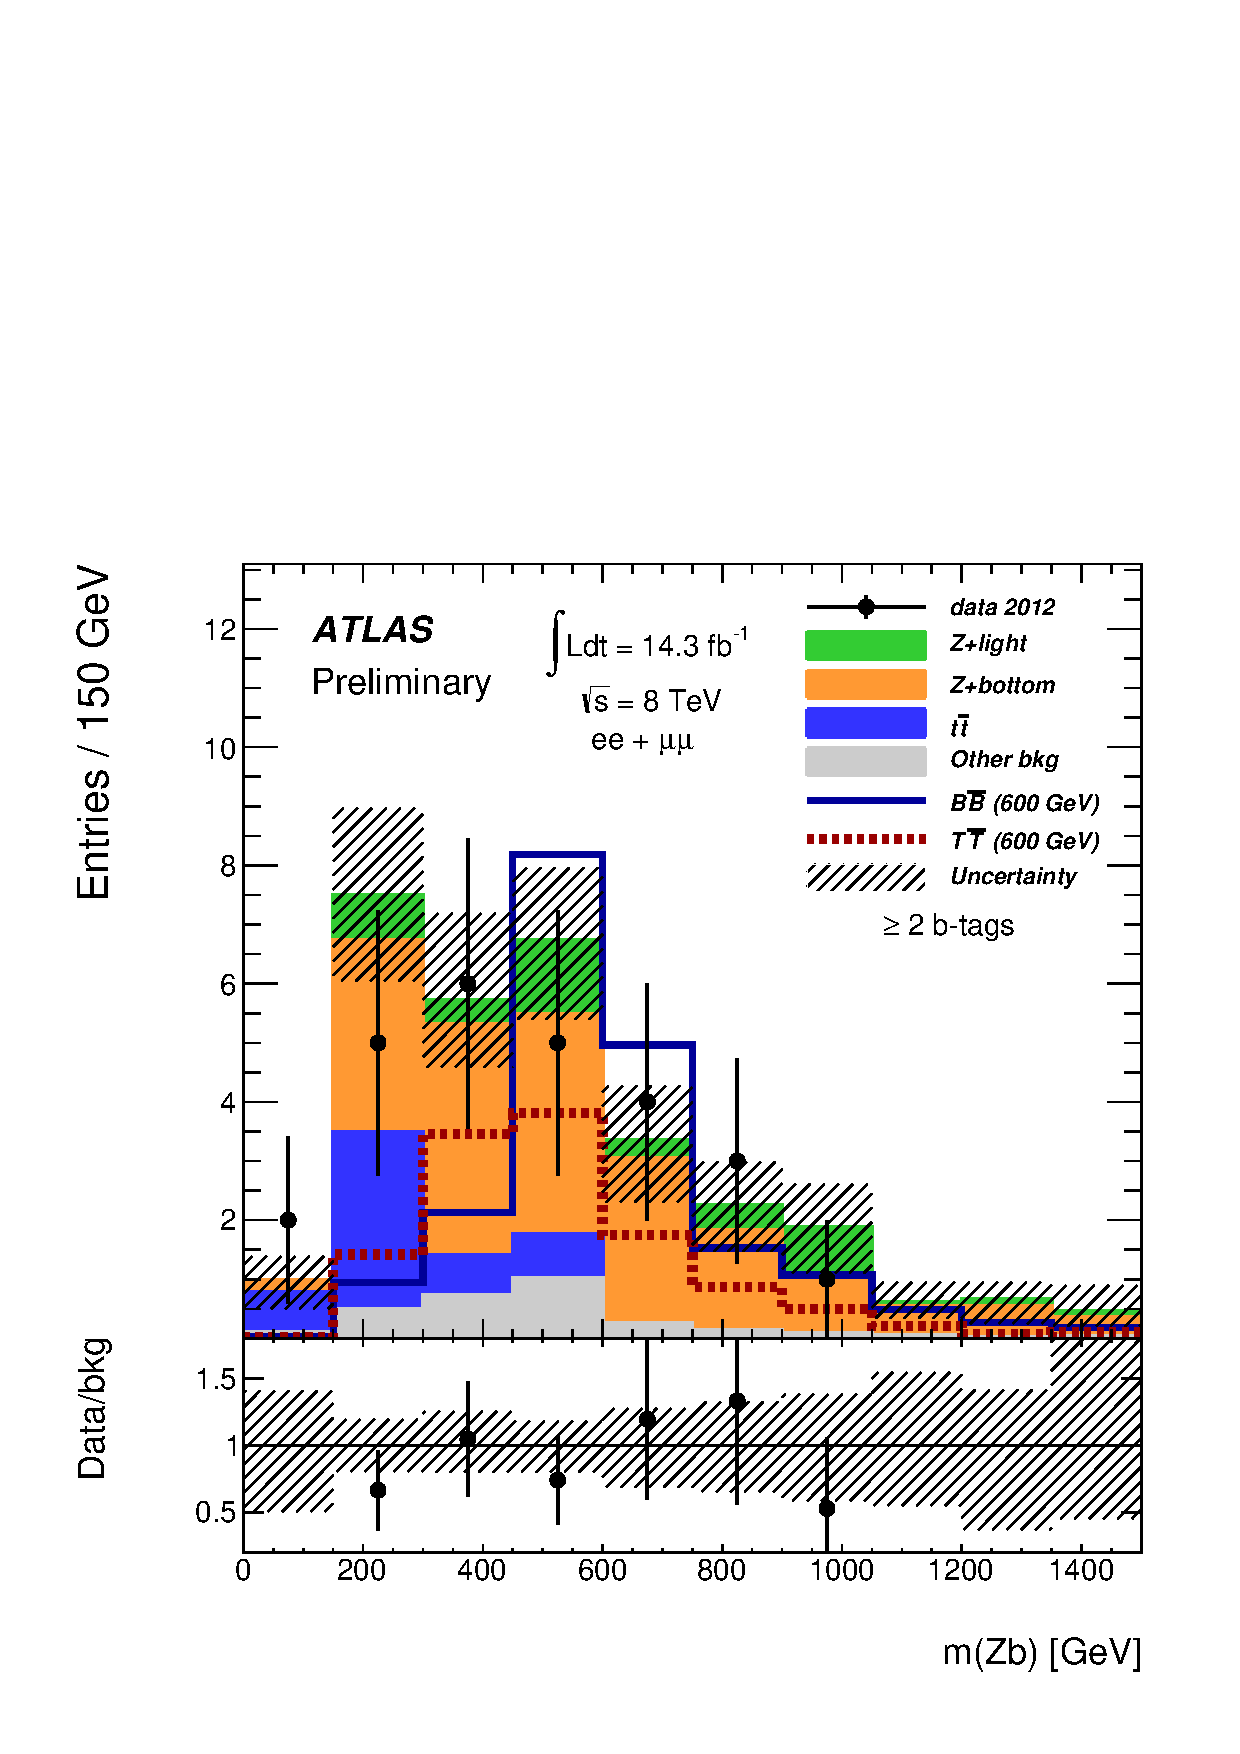
\includegraphics[width=.9\textwidth]{ztag/fig_07b}
\scriptsize

$m(Zb)$ is the final test variable:\\
invariant mass of the $Z$ candidate\\
paired with the highest $p_T$ $b$-tagged jet

\end{minipage}

\end{frame}


\begin{frame}\frametitle{$T$ exclusion plane~\cite{combination} III}
\footnotesize\centering

\includegraphics[width=1.\textwidth]{comb2d/ATLAS_VLQ_TT_june2013_step3}

\end{frame}


\begin{frame}\frametitle{$B$ exclusion plane~\cite{combination} II}
\footnotesize\centering

\includegraphics[width=1.\textwidth]{comb2d/ATLAS_VLQ_BB_june2013_step2}

\end{frame}



%%%%%%%%%%%%%%%%%%%%%%%%%%%%%%
\section{$T\bar{T}\to Wb+X$}
%%%%%%%%%%%%%%%%%%%%%%%%%%%%%%
\begin{frame}\frametitle{$T\bar{T}\to Wb+X\qquad$\small ATLAS-CONF-2013-060~\cite{ATLAS-CONF-2013-060} \tiny $\;$ update of~\cite{ATLAS:2012qe}}
\footnotesize\centering

Exploit $T$'s boosted kinematics to reconstruct $W$ bosons \scriptsize
  \begin{minipage}{.65\textwidth}\centering


  \begin{minipage}{.45\textwidth}\centering

\begin{pgfpicture}{0.0\textwidth}{0.0\textheight}{1.\textwidth}{.6\textwidth}
   \begin{pgftranslate}{\pgfpoint{0.05\textwidth}{-0.12\textheight}}
\pgfdeclareimage[interpolate=true,width=.95\textwidth]{mindr}{wbx/fig_05b.pdf}
\pgfputat{\pgfxy(0.0,0.0)}{\pgfbox[left,base]{\pgfuseimage{mindr}}}
 \pgfsetlinewidth{1.pt}
 \usebeamercolor[bg]{head/foot boxes}
 \pgfline{\pgfxy(1.55,0.35)}{\pgfxy(1.55,2.5)} 
 \pgfstroke
 \pgfsetendarrow{\pgfarrowlargepointed{6pt}}
 \pgfline{\pgfxy(2.4,1.6)}{\pgfxy(3.6,2.)}
 \pgfstroke
   \end{pgftranslate}

\end{pgfpicture}


\myskip
\myskip
\myskip

    \begin{itemize}
    \item \alert{$W^{type I}_{had}$}: {\tiny single merged jet ($p_T>250~$GeV, $m_{j}\in [60,120]~$GeV)}
    \item \alert{$W^{type II}_{had}$}: {\tiny two close-by jets ($\Delta R(j,j)<0.8$, $p_T>200~$GeV,  $m_{jj}\in [60,120]~$GeV)}
    \end{itemize}


  \end{minipage}\begin{minipage}{.55\textwidth}
\centering\tiny
      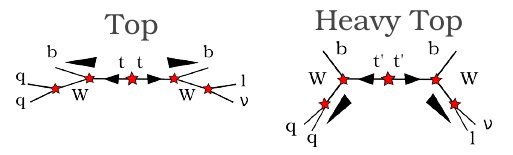
\includegraphics[width=1.\textwidth]{wbx/boost}

    \begin{itemize}
    \item $\Delta R(l,\nu) < 1.2$
    \item $min(\Delta R(l,b_{1,2})) > 1.4$
    \item $min(\Delta R(W_{had},b_{1,2})) > 1.4$
    \end{itemize}

     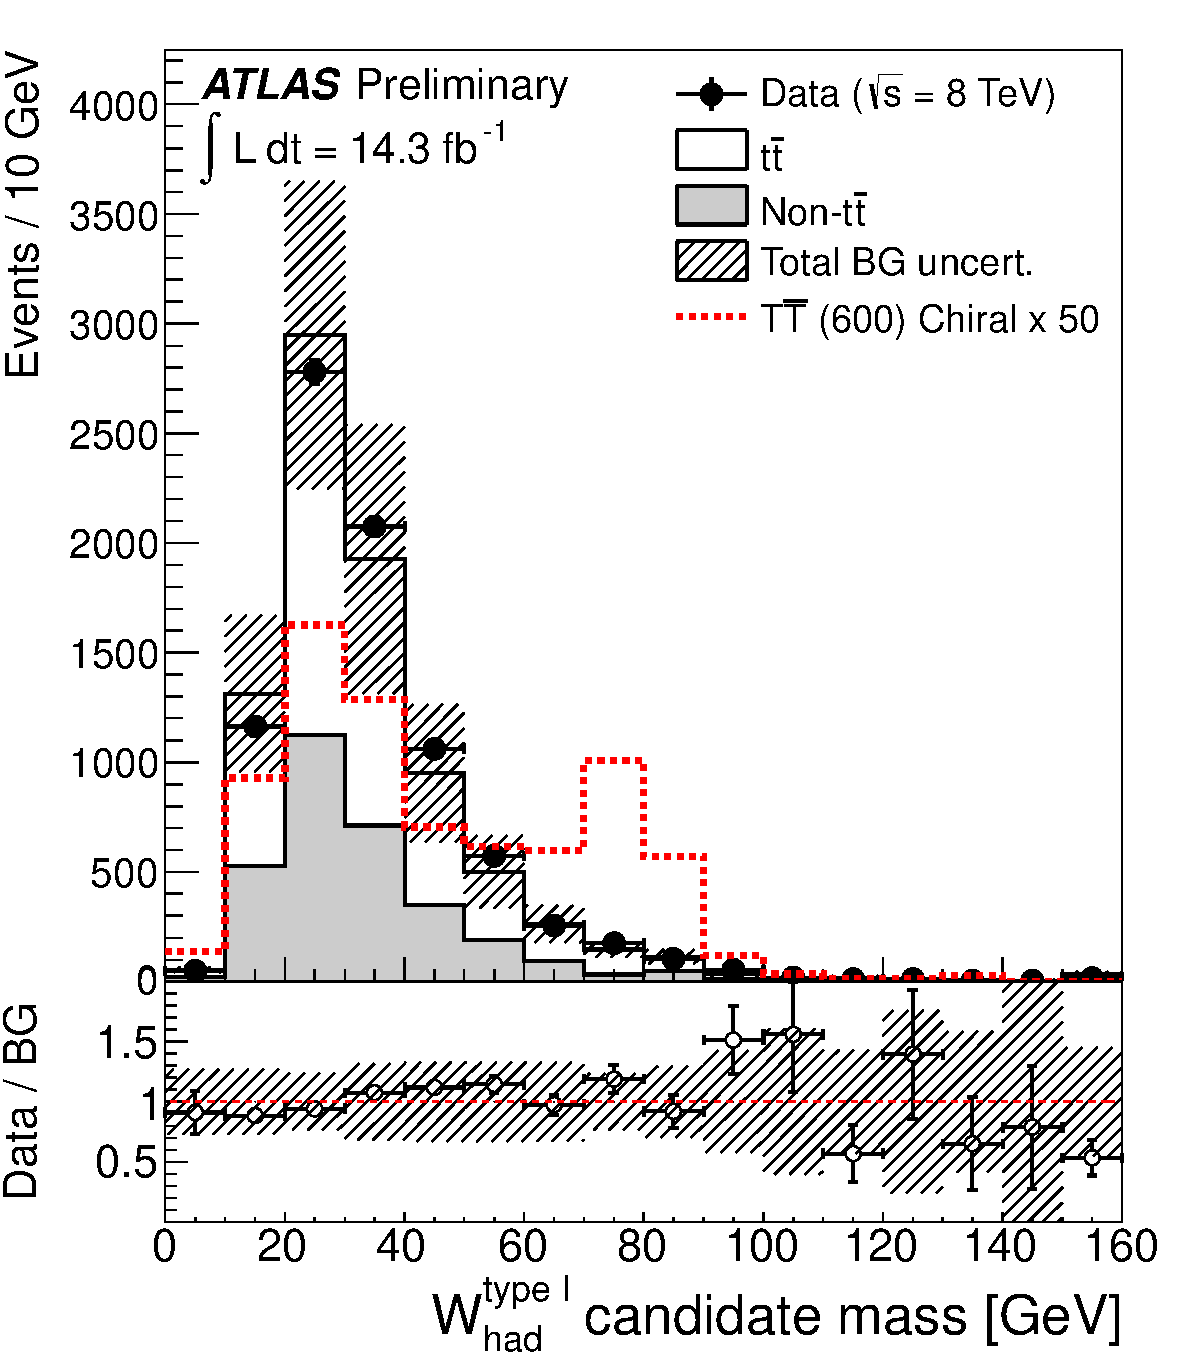
\includegraphics[width=.8\textwidth]{wbx/fig_02a.pdf}

  \end{minipage}

%


    \end{minipage}\begin{minipage}{.35\textwidth}
\centering\scriptsize

      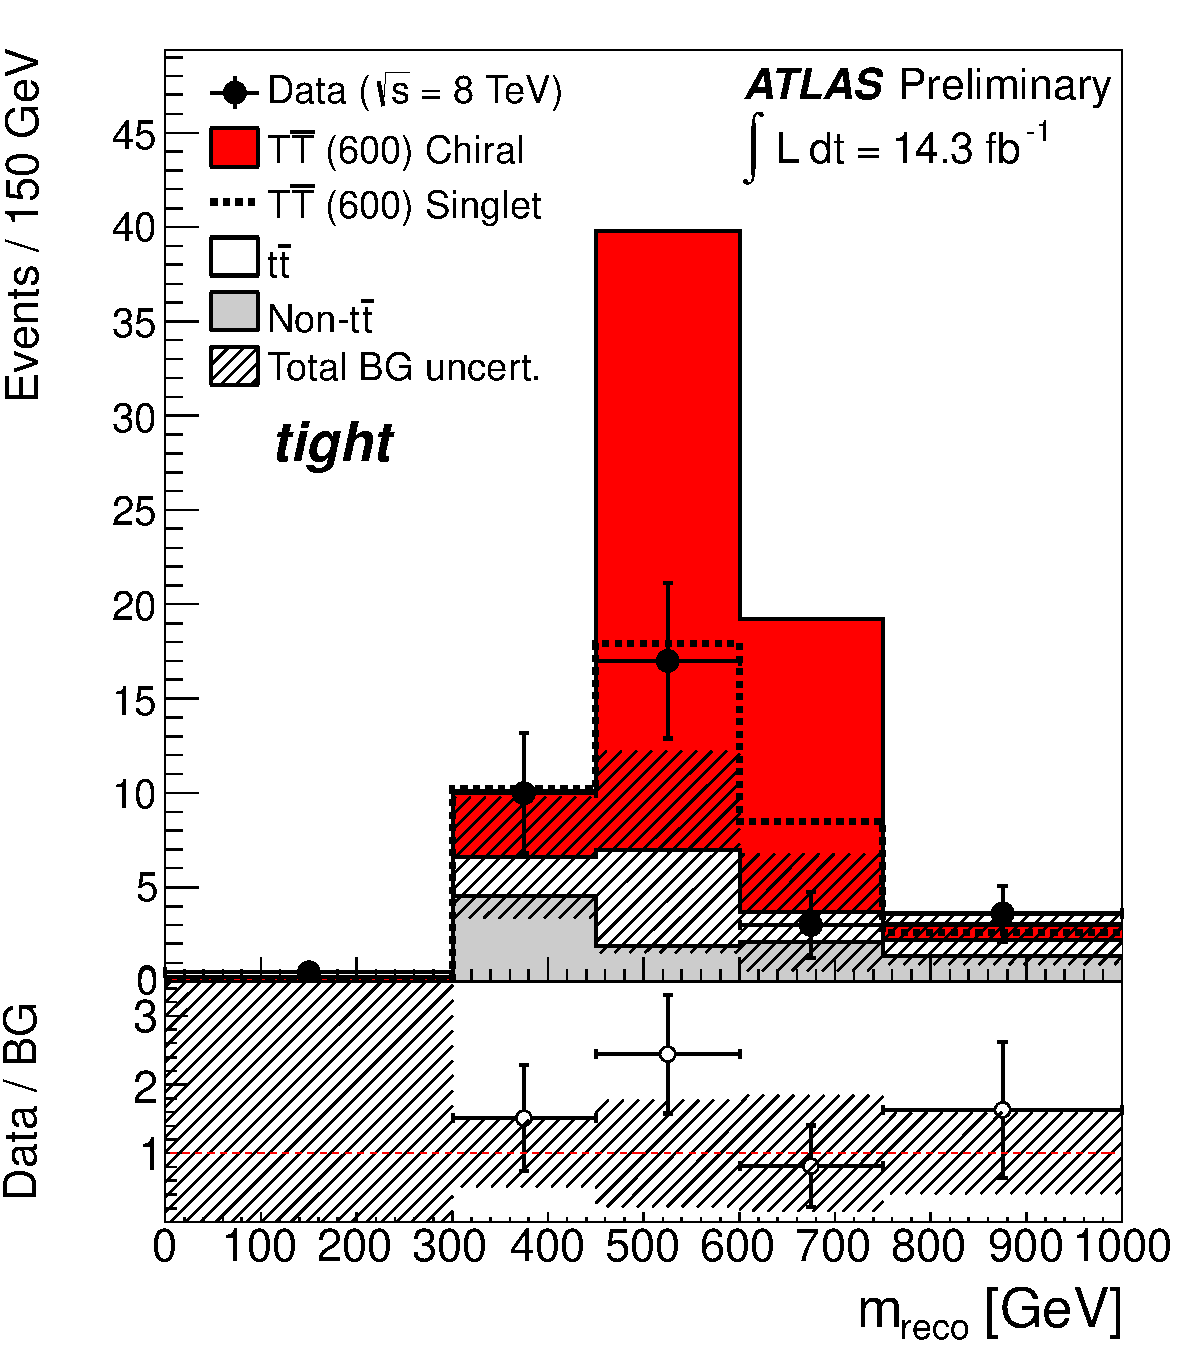
\includegraphics[width=1.\textwidth]{wbx/fig_06b.pdf}

The reconstructed $W$ boson is matched to the $b$-tagged jets that gives the lowest mass difference between the leptonical and hadronical leg
    \end{minipage}

\end{frame}

\begin{frame}\frametitle{$T$ exclusion plane~\cite{combination} IV}
\footnotesize\centering

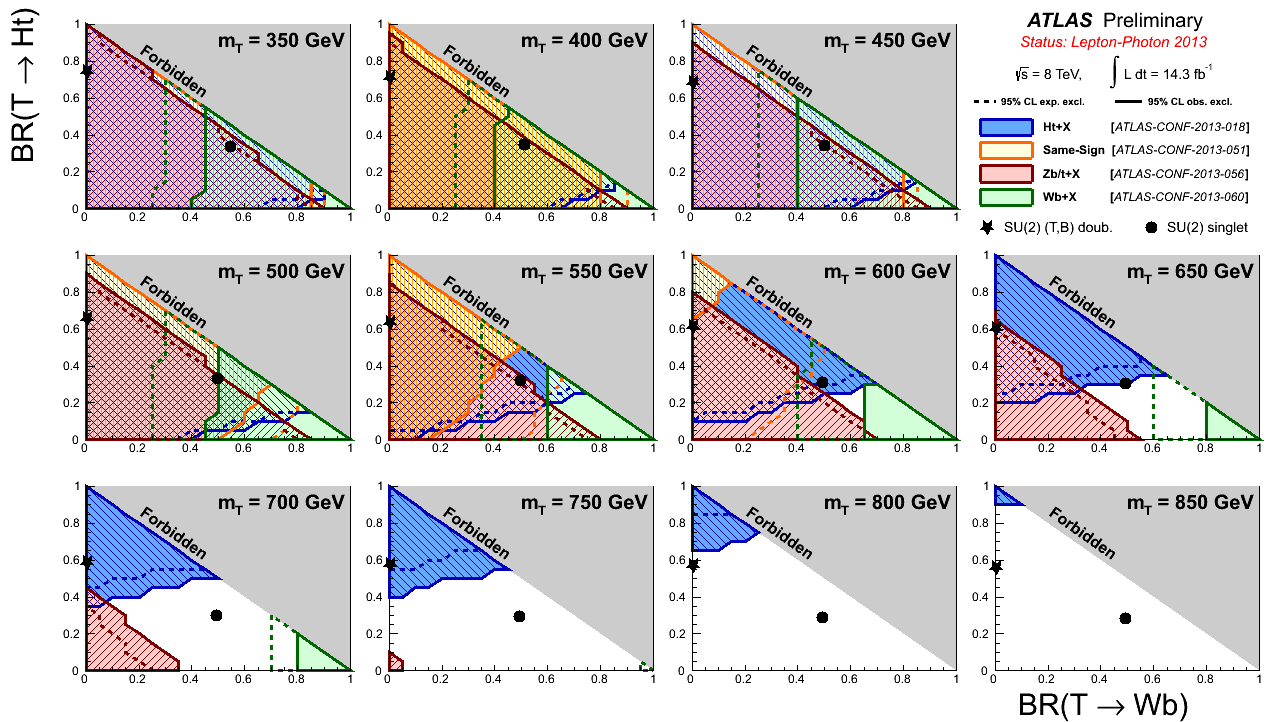
\includegraphics[width=1.\textwidth]{comb2d/ATLAS_VLQ_TT_june2013_step4}

\end{frame}



%%%%%%%%%%%%%%%%
\section{Conclusions}
%%%%%%%%%%%%%%%%
\begin{frame}\frametitle{Conclusions}
\scriptsize\centering

\begin{minipage}{.32\textwidth}
Using 14\ifb\ of $\sqrt{s}=8~$TeV 2012 LHC data, ATLAS performed four preliminary \alert{model independent} and \alert{complementary} searches for heavy quarks

\centering

\begin{itemize}
\item Updating $\sqrt{s}=7~$TeV analyses
\end{itemize}


Considering a few benchmark points, at 95\% CL we exclude:
\begin{itemize}
\item Singlet $T$ with mass up to 670~GeV~\cite{ATLAS-CONF-2013-018,ATLAS-CONF-2013-060}
\item Singlet $B$ with mass up to 645~GeV~\cite{ATLAS-CONF-2013-056}
\item Doublet $T$ with mass up to 790~GeV~\cite{ATLAS-CONF-2013-018}
\item Doublet $B$ with mass up to 725~GeV~\cite{ATLAS-CONF-2013-056}
\end{itemize}


\end{minipage}\begin{minipage}{.68\textwidth}
\centering
\vskip-6ex
\begin{minipage}{.5\textwidth}\centering
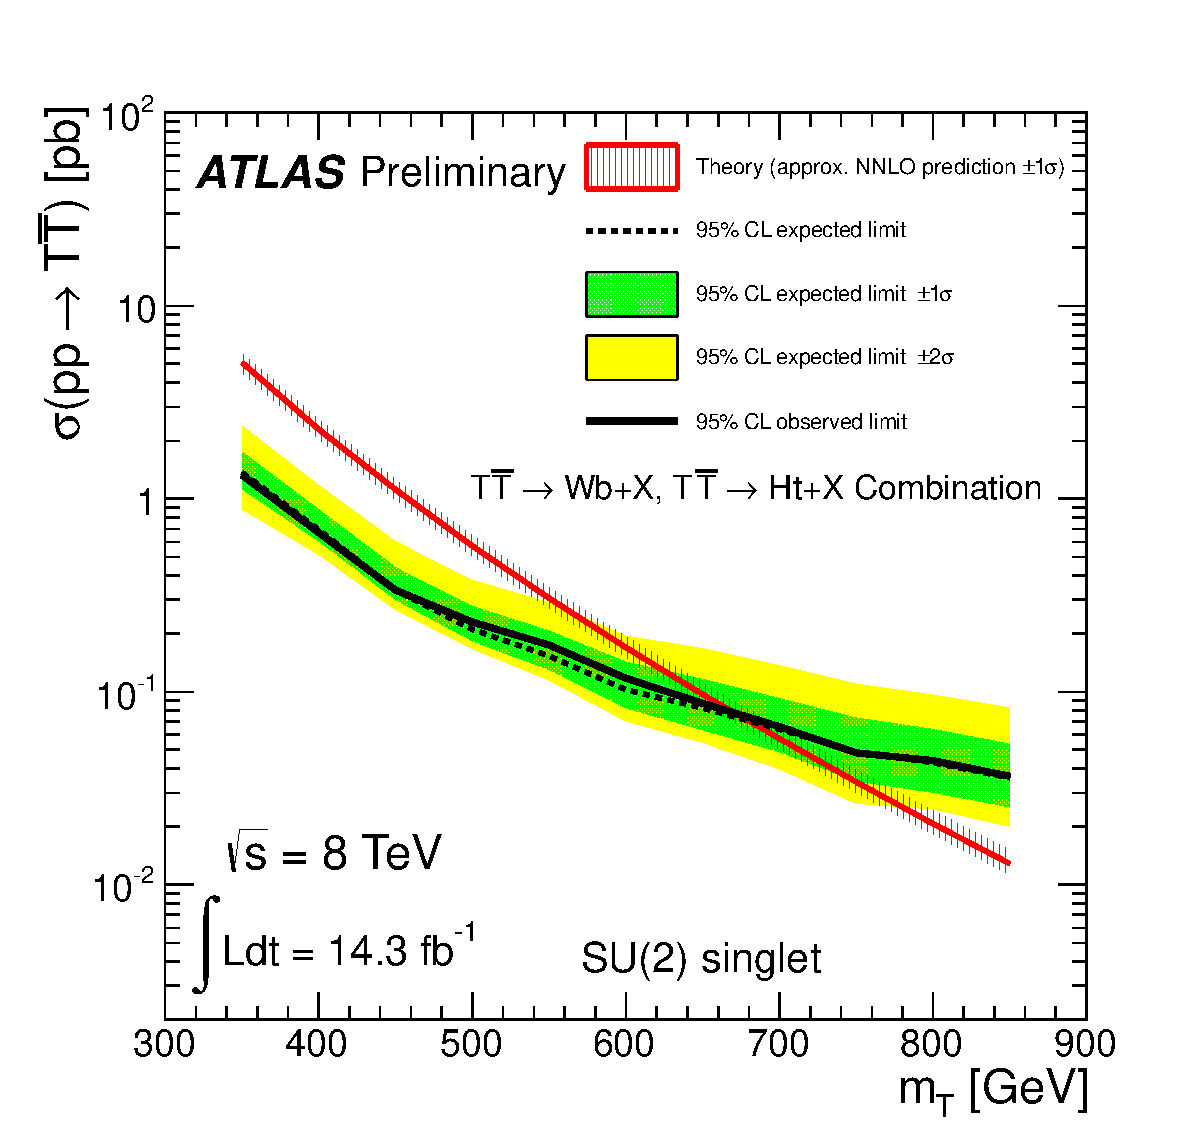
\includegraphics[width=1.\textwidth]{wbx/fig_09}
\end{minipage}\begin{minipage}{.5\textwidth}\centering
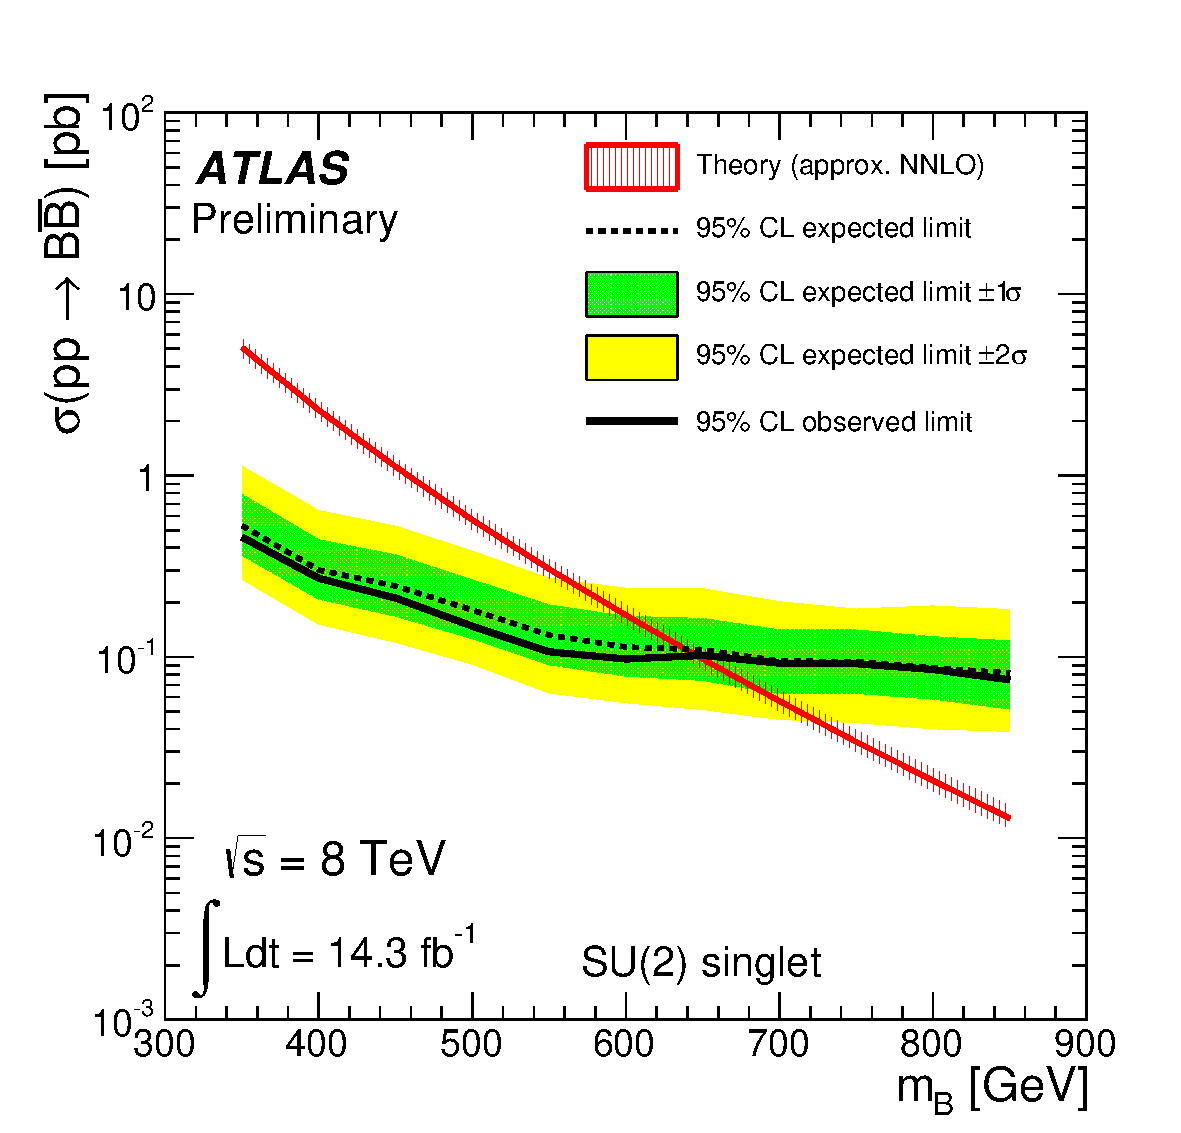
\includegraphics[width=1.\textwidth]{ztag/fig_08a}
\end{minipage}

\begin{minipage}{.5\textwidth}\centering
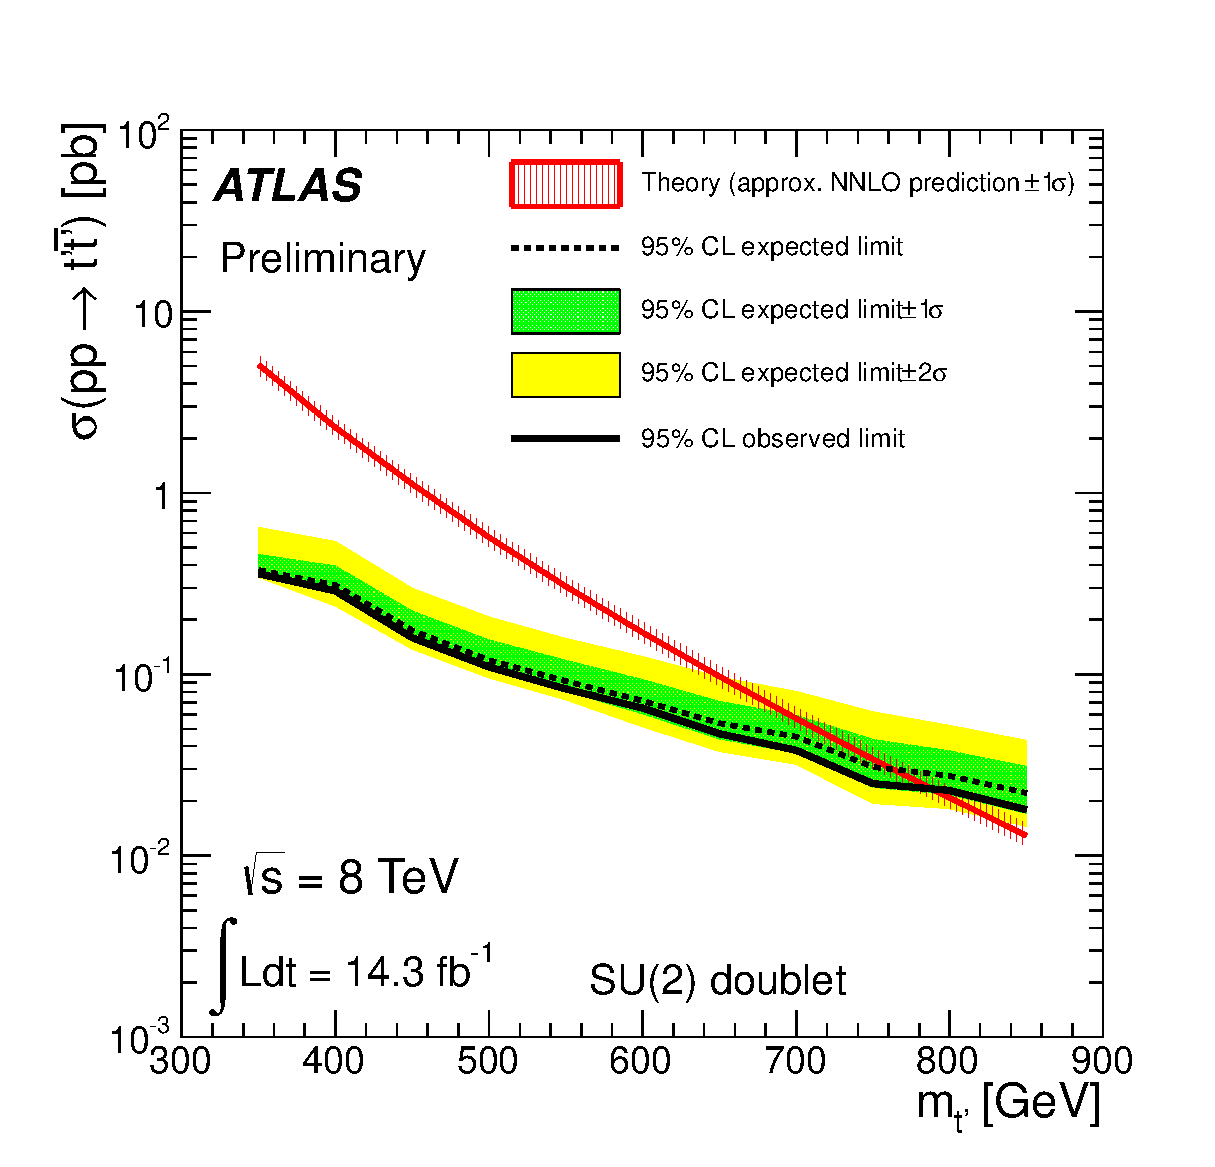
\includegraphics[width=1.\textwidth]{htx/fig_05a}
\end{minipage}\begin{minipage}{.5\textwidth}\centering
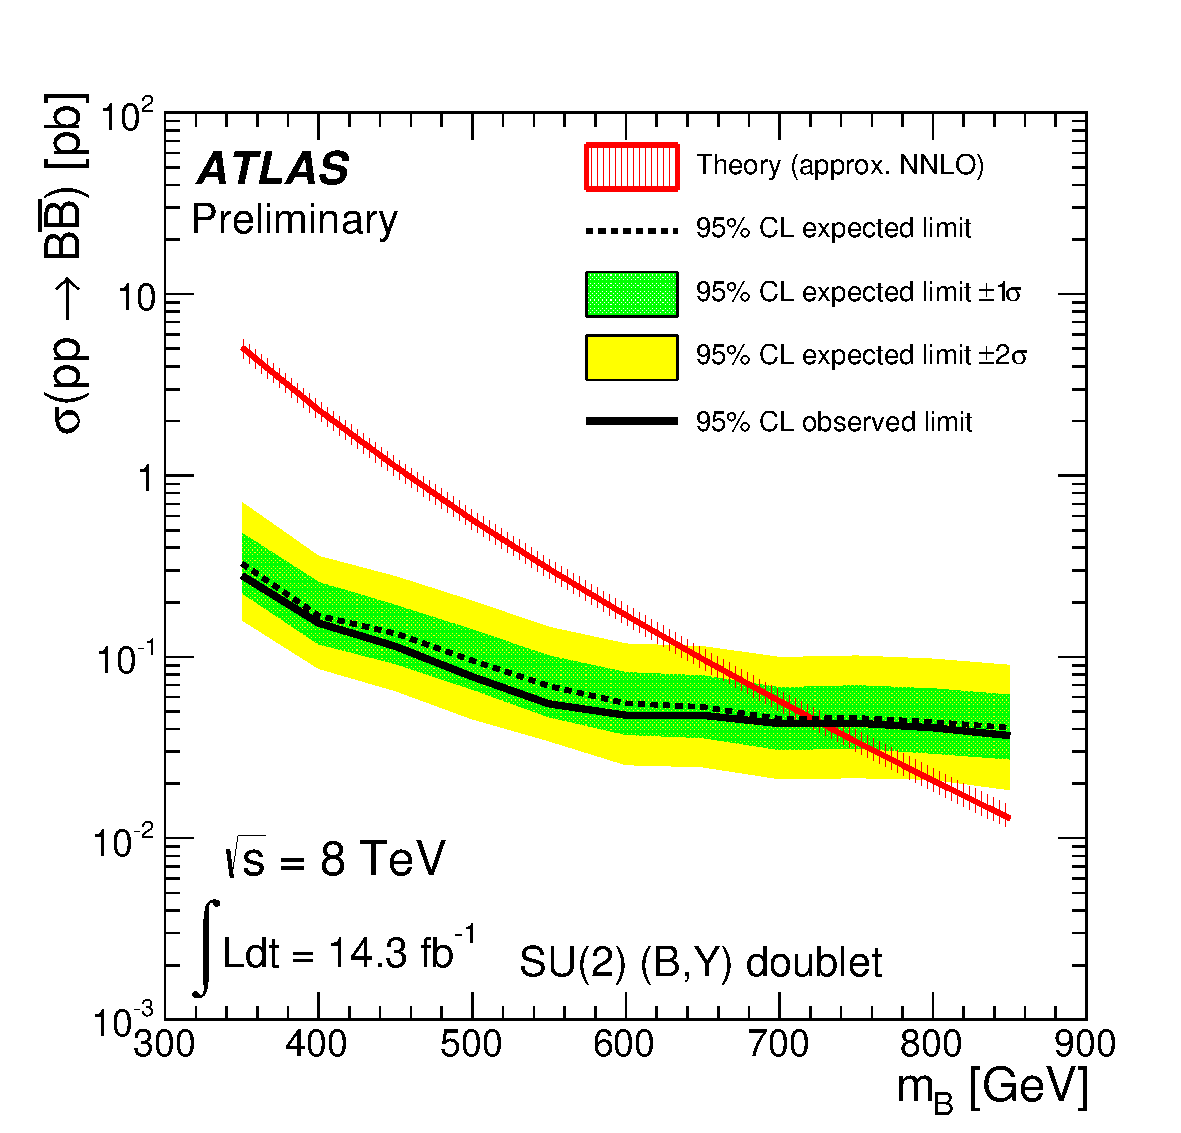
\includegraphics[width=1.\textwidth]{ztag/fig_08b}
\end{minipage}




\end{minipage}

\end{frame}



\appendix


\section*{References}
\setbeamertemplate{bibliography item}[text]

\begin{frame}[allowframebreaks]
\frametitle{References}\footnotesize
\bibliographystyle{unsrt}
%\bibliographystyle{myunsrt}
\bibliography{heavyquarks.bib}
\end{frame}


\section*{Backup}

%----------------------------------
\begin{frame}
 \frametitle{}

\begin{center}{\bfseries
BACKUP SLIDES}
\end{center}
\end{frame}



\begin{frame}\frametitle{Event preselection}
\footnotesize\centering

ATLAS working groups defined standard object definitions\\
analyses use in general these definitions, as well as common selections\\

\myskip

\begin{minipage}{.5\textwidth}
\centering
\alert{Object definitions}

\begin{itemize}\scriptsize
\item \alert{Jets}: Topological clusters reconstructed with the \texttt{AntikT4} algorithm ($p_T > $25~GeV, $|\eta|<$2.5, JVF$>0.5^{(a)}$) 
\item \alert{Electrons}: Well isolated calo object matched to track ($E_T>$25~GeV, $|\eta|$ in [0,2.47] removing [1.37,1.52], $z_0<2~$mm$^{(b)}$)
\item \alert{Muons}: Segment in the tracker and muon detector, isolated track ($p_T>$ 25~GeV, $|\eta|<$2.5, $z_0<2~$mm$^{(b)}$)
\end{itemize}
\scriptsize
If jets within $\Delta R < 0.2$ of an electron, the closest jet is discarded; Leptons within $\Delta R < 0.4$ of a jet are removed

\end{minipage}\begin{minipage}{.5\textwidth}
\centering


\alert{Event pre-selection}
\begin{itemize}\scriptsize
\item $\geq$ 5 tracks from the Primary Vertex (Cosmics and Pileup rejection)
\item If more vertices, choose the one with largest sum of $p_T^2$
\item Single lepton triggers: isolated electron with $p_T>24~$GeV OR electron with $p_T>60~$GeV OR isolated muon with $p_T>24~$GeV OR muon with $p_T>36~$GeV
\end{itemize}
\scriptsize
\myskip
If the analysis requires one or more leptons, at least one of them must match the single lepton trigger


\end{minipage}

\myskip

\tiny
$^{(a)}$ the jet vertex fraction is defined as the fraction of summed $p_T$ ($>0.5~$GeV) of tracks associated to the jet that come from the primary vertex\\
$^{(b)}$ $z_0$ is the longitudinal impact parameter of the track wrt the primary vertex


\end{frame}





\begin{frame}\frametitle{$T\bar{T}\to Ht+X$~\cite{ATLAS-CONF-2013-018}}
\footnotesize\centering

       Three channels:\\ $=2$, $=3$, \alert{$\geq 4$ $b$-tagged jets}

       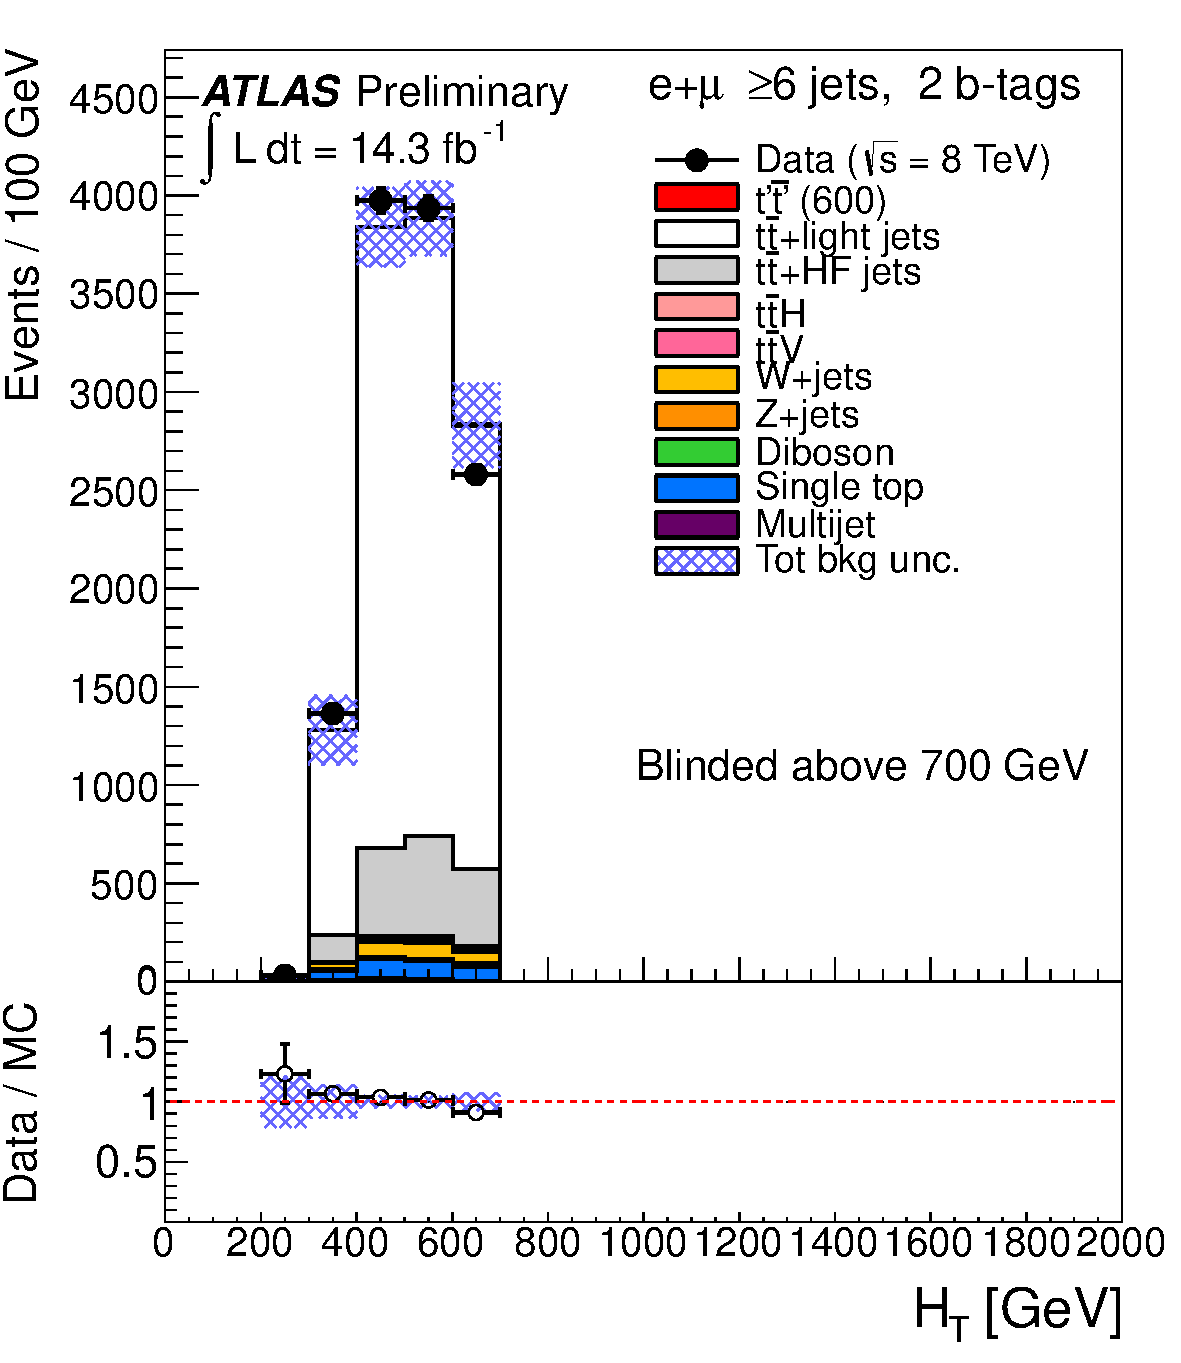
\includegraphics[width=.33\textwidth]{htx/fig_04a.pdf}
       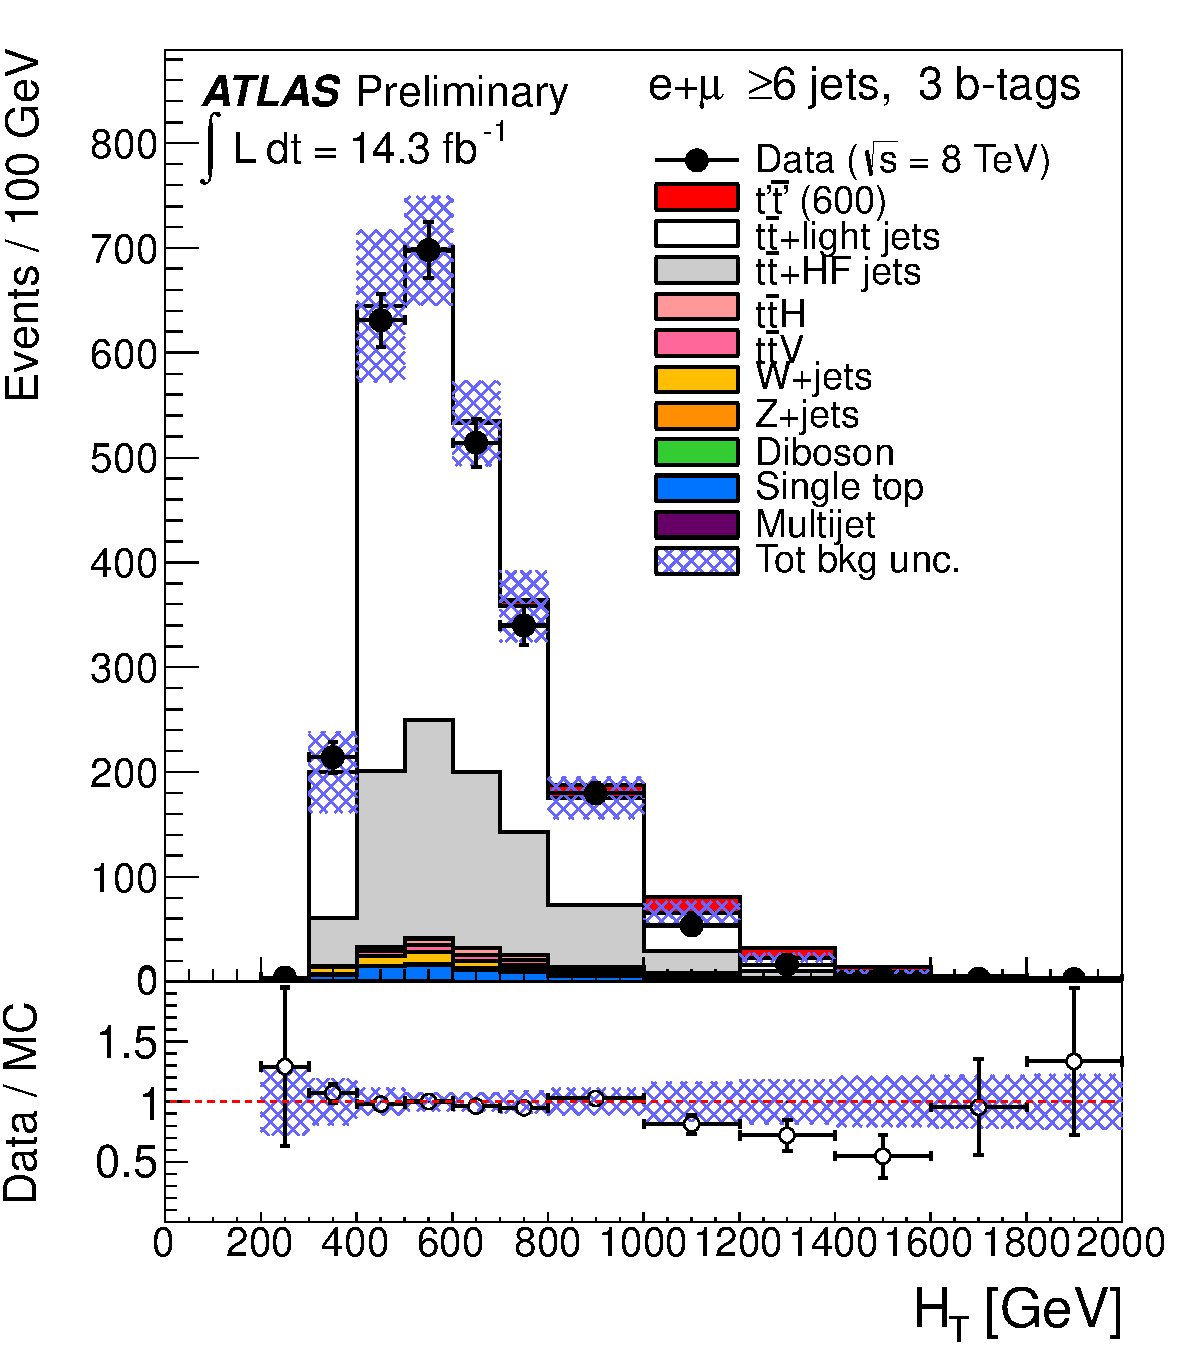
\includegraphics[width=.33\textwidth]{htx/fig_04b.pdf}
       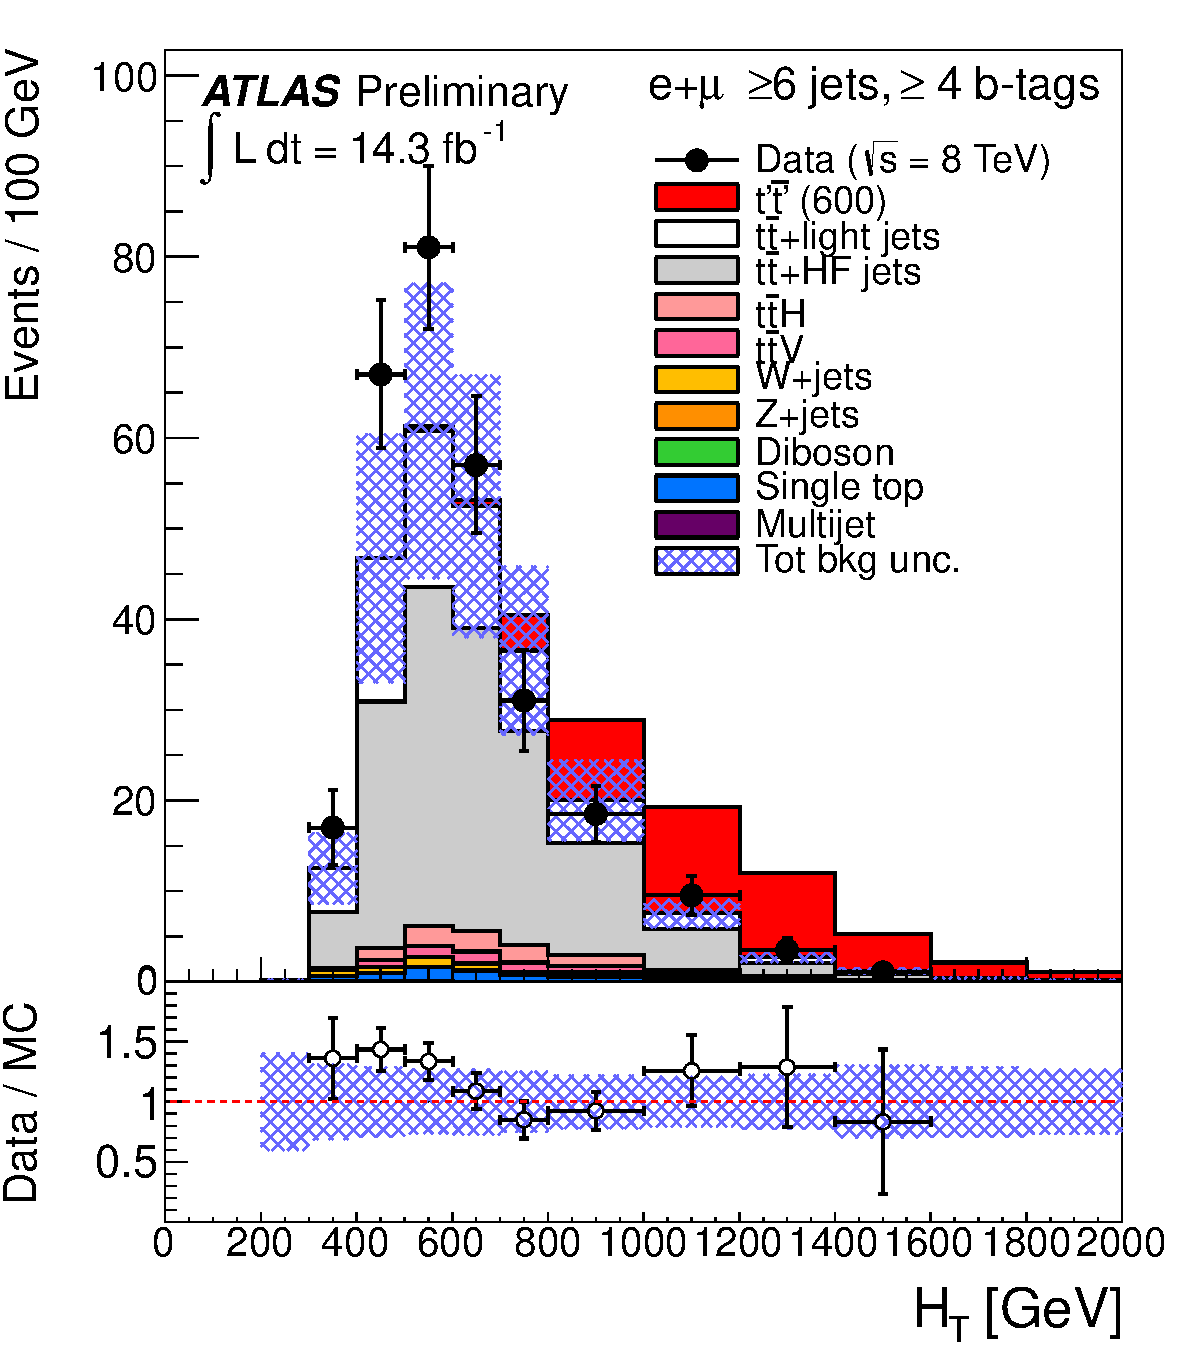
\includegraphics[width=.33\textwidth]{htx/fig_04c.pdf}

\end{frame}


\begin{frame}\frametitle{$T\bar{T}\to Ht+X$~\cite{ATLAS-CONF-2013-018}}
\footnotesize\centering

       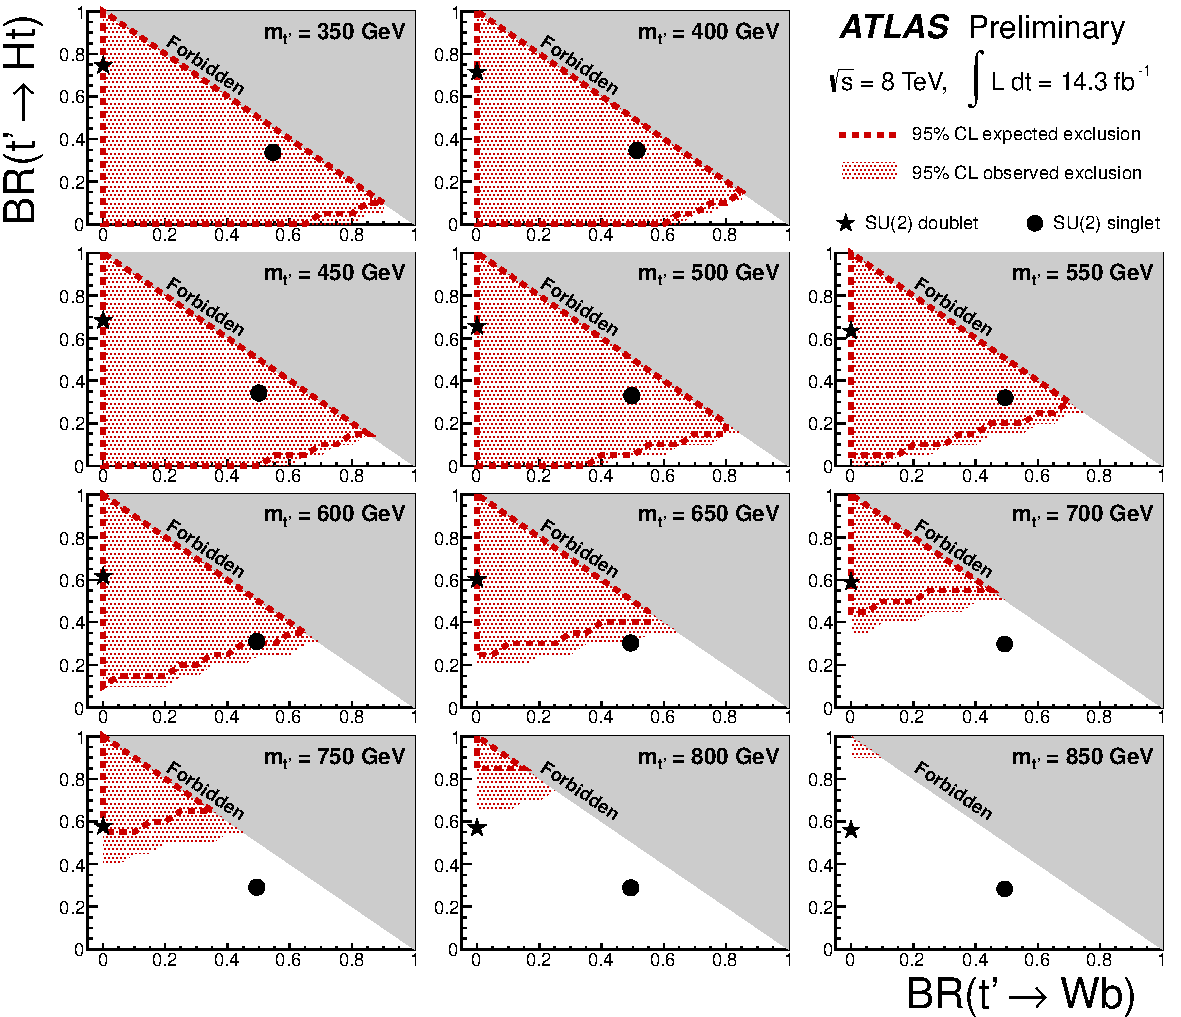
\includegraphics[width=.7\textwidth]{htx/fig_06.pdf}

\end{frame}

\begin{frame}\frametitle{Same-sign dileptons~\cite{ATLAS-CONF-2013-051}}
\footnotesize\centering

       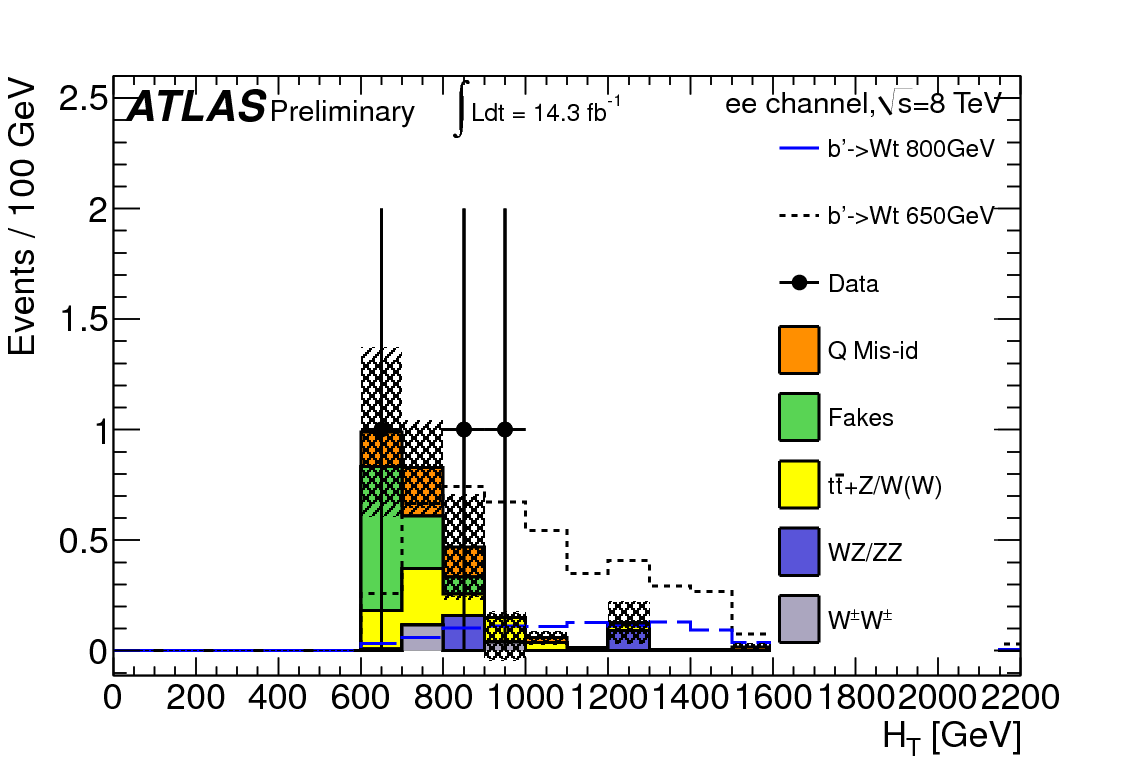
\includegraphics[width=.33\textwidth]{ssign/fig_03a}
       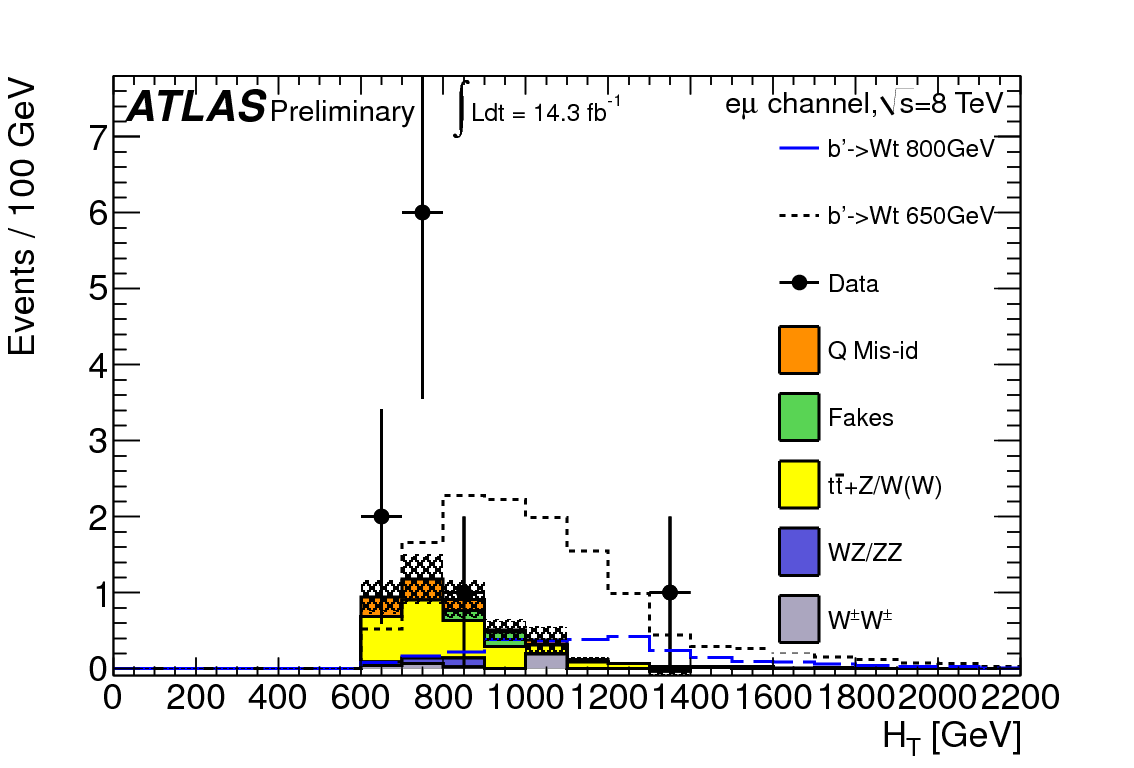
\includegraphics[width=.33\textwidth]{ssign/fig_03c}
       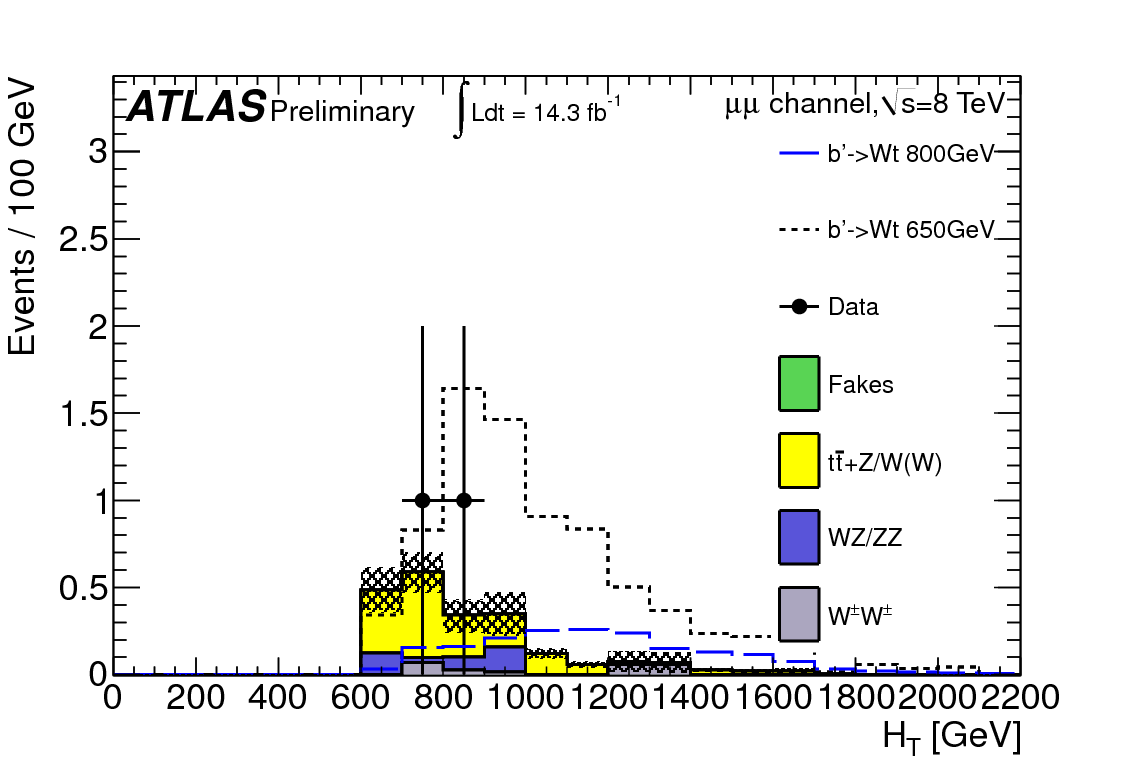
\includegraphics[width=.33\textwidth]{ssign/fig_03e}

       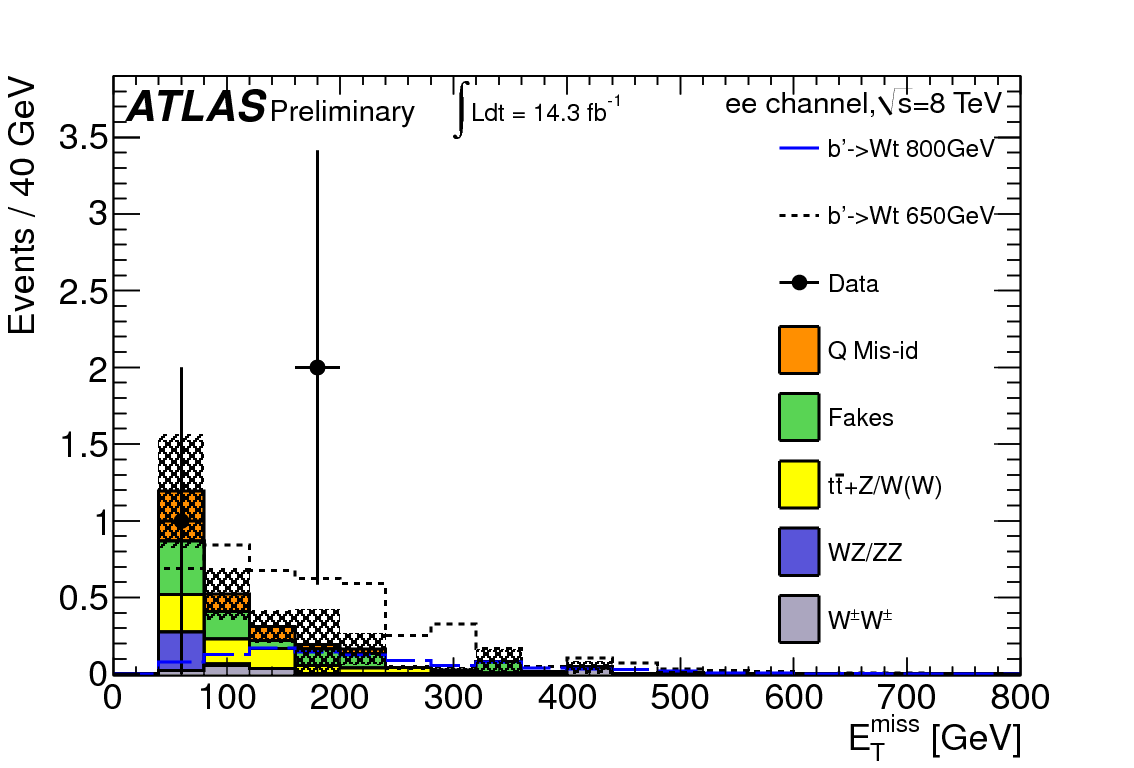
\includegraphics[width=.33\textwidth]{ssign/fig_03b}
       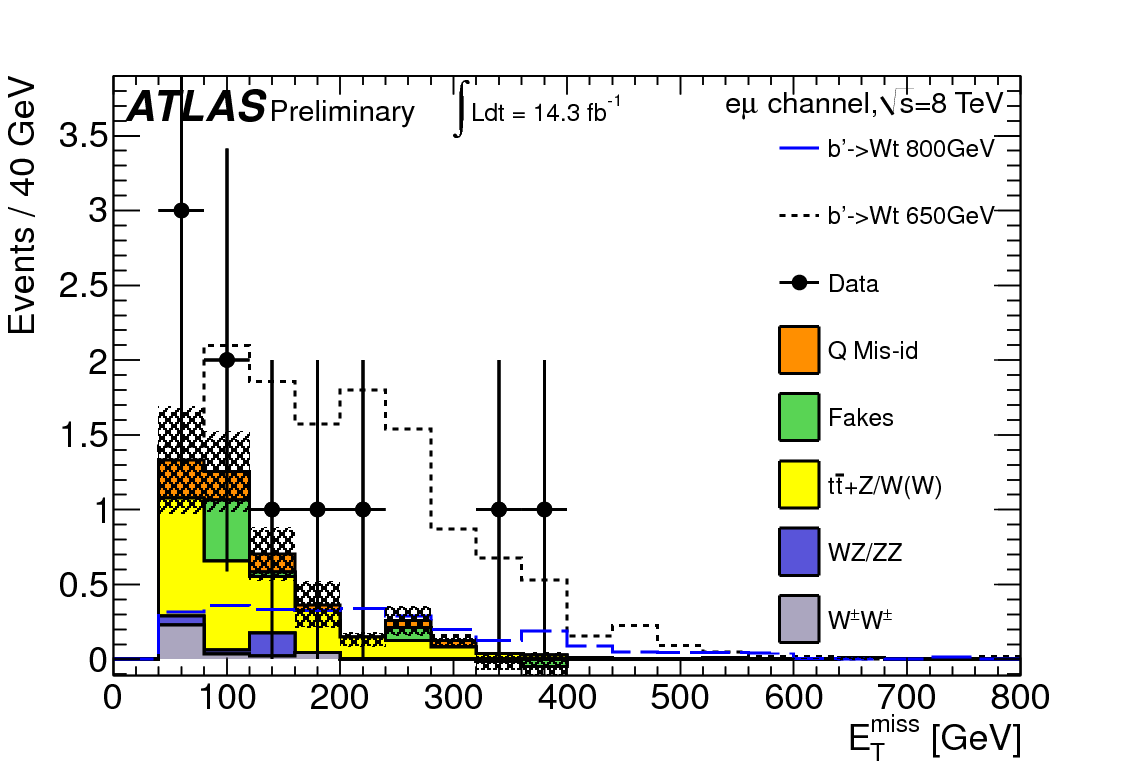
\includegraphics[width=.33\textwidth]{ssign/fig_03d}
       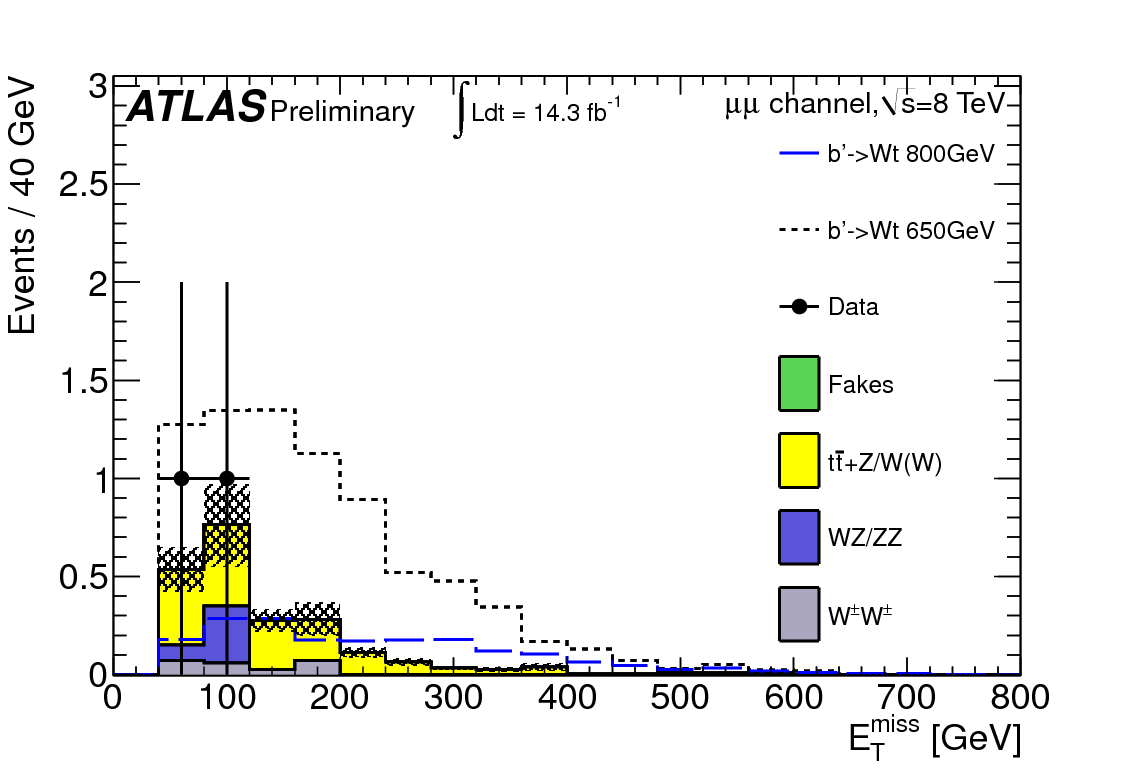
\includegraphics[width=.33\textwidth]{ssign/fig_03f}

\end{frame}


\begin{frame}\frametitle{Same-sign dileptons~\cite{ATLAS-CONF-2013-051}}
\footnotesize\centering

       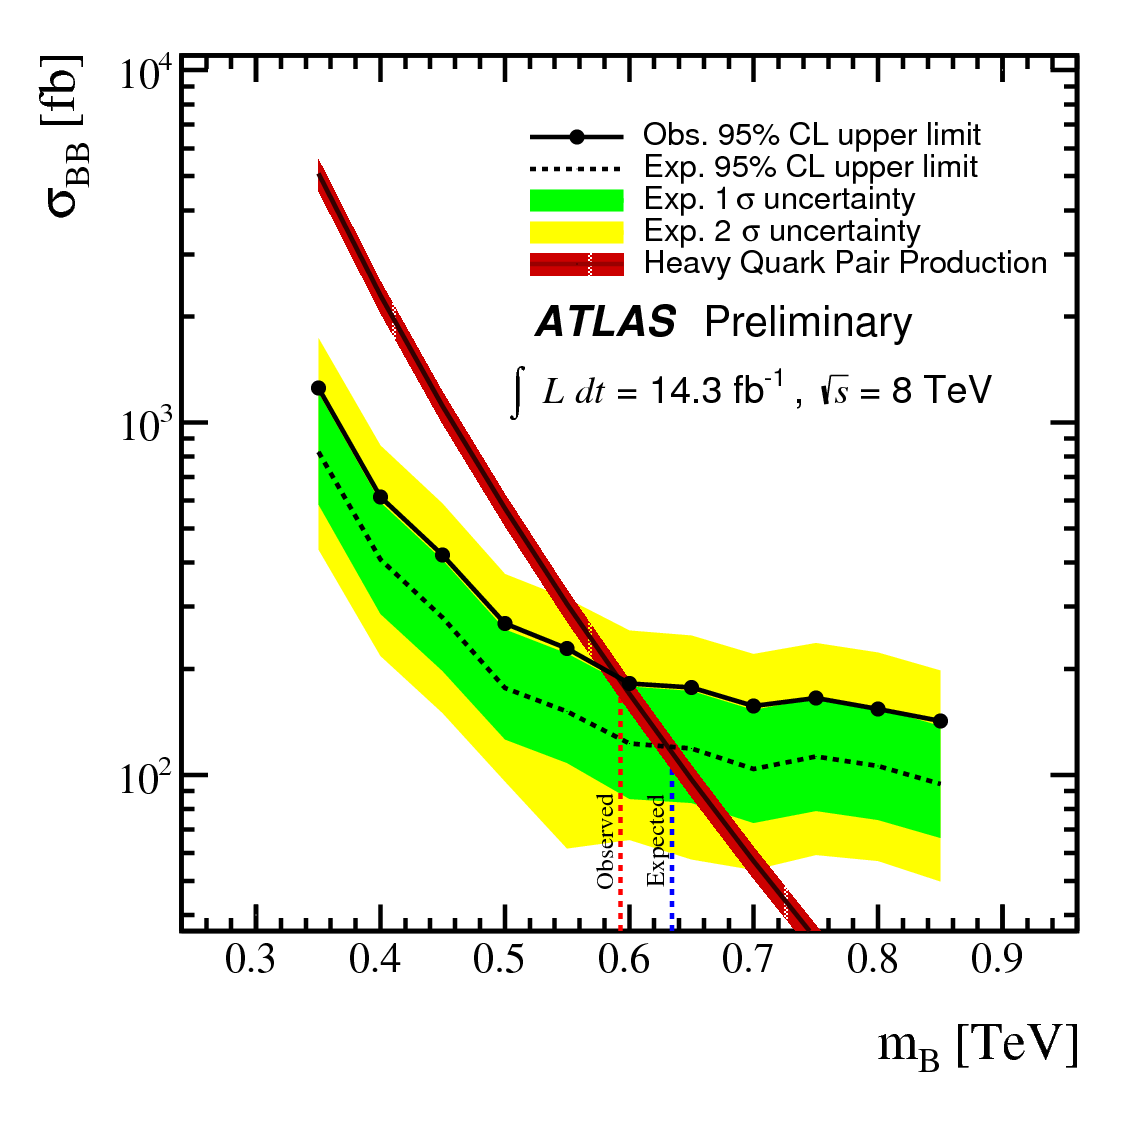
\includegraphics[width=.5\textwidth]{ssign/fig_06a}
       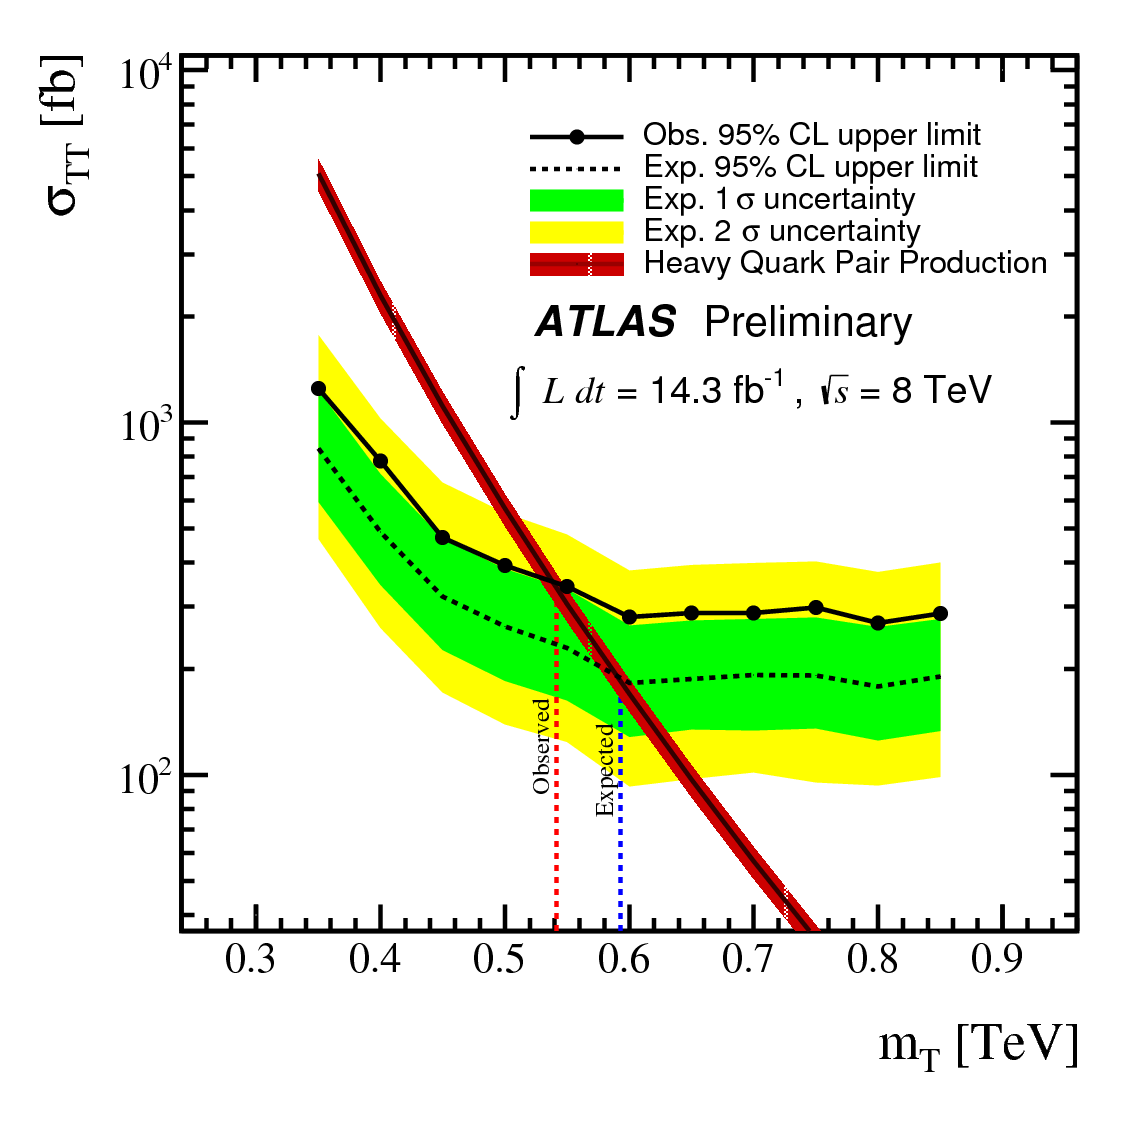
\includegraphics[width=.5\textwidth]{ssign/fig_06b}

\end{frame}

\begin{frame}\frametitle{Same-sign dileptons~\cite{ATLAS-CONF-2013-051}}
\footnotesize\centering

       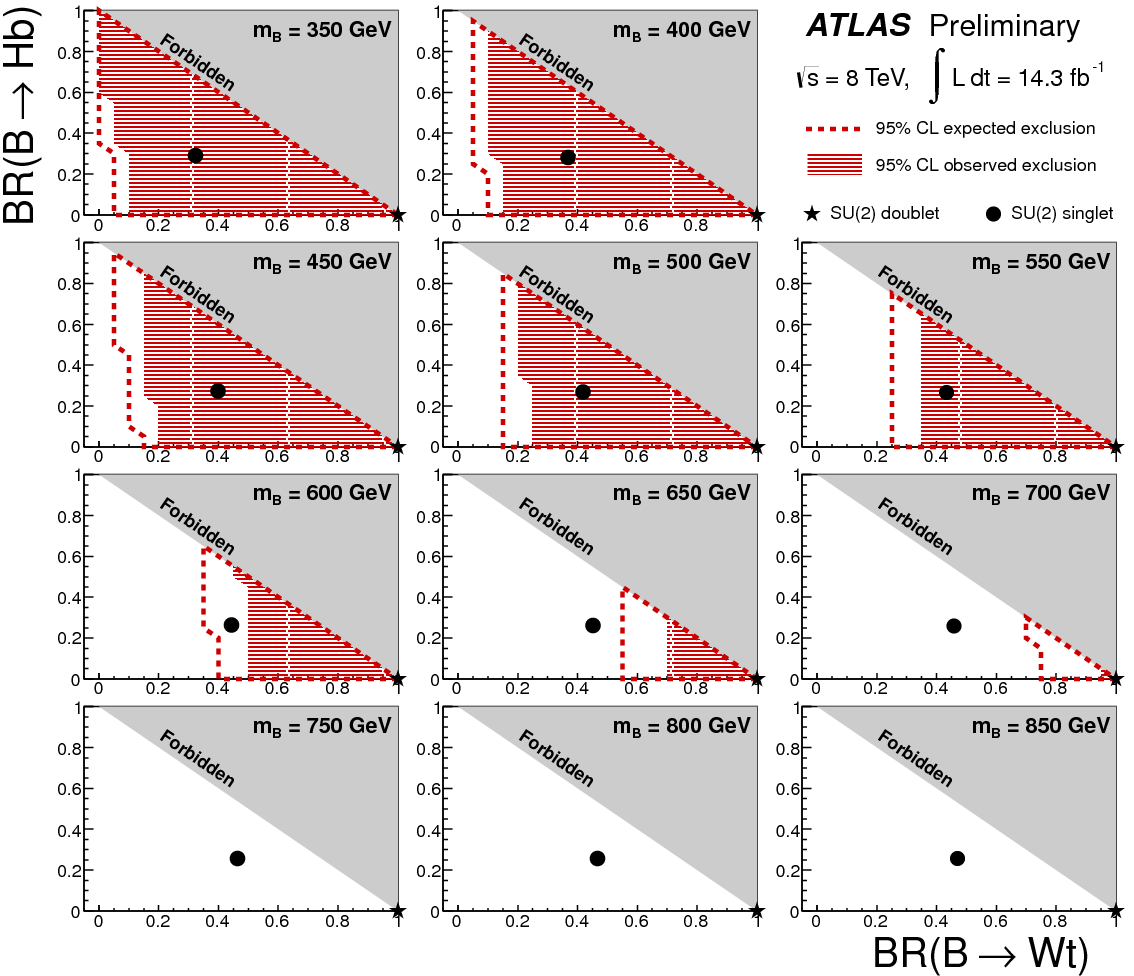
\includegraphics[width=.7\textwidth]{ssign/fig_07}

\end{frame}

\begin{frame}\frametitle{Same-sign dileptons~\cite{ATLAS-CONF-2013-051}}
\footnotesize\centering

       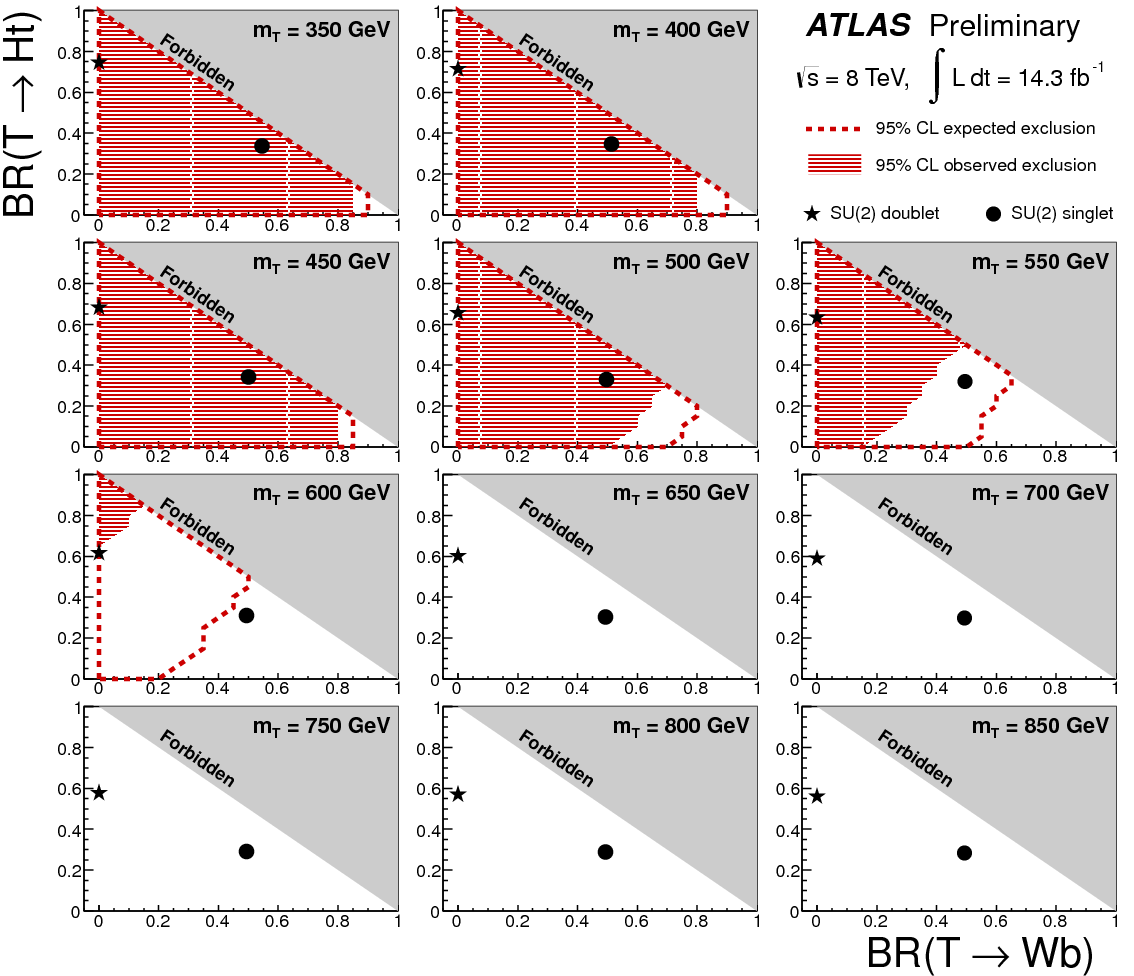
\includegraphics[width=.7\textwidth]{ssign/fig_08}

\end{frame}





\begin{frame}\frametitle{$B\bar{B}(T\bar{T})\to Zb(t)+X$~\cite{ATLAS-CONF-2013-056}}
\footnotesize\centering

       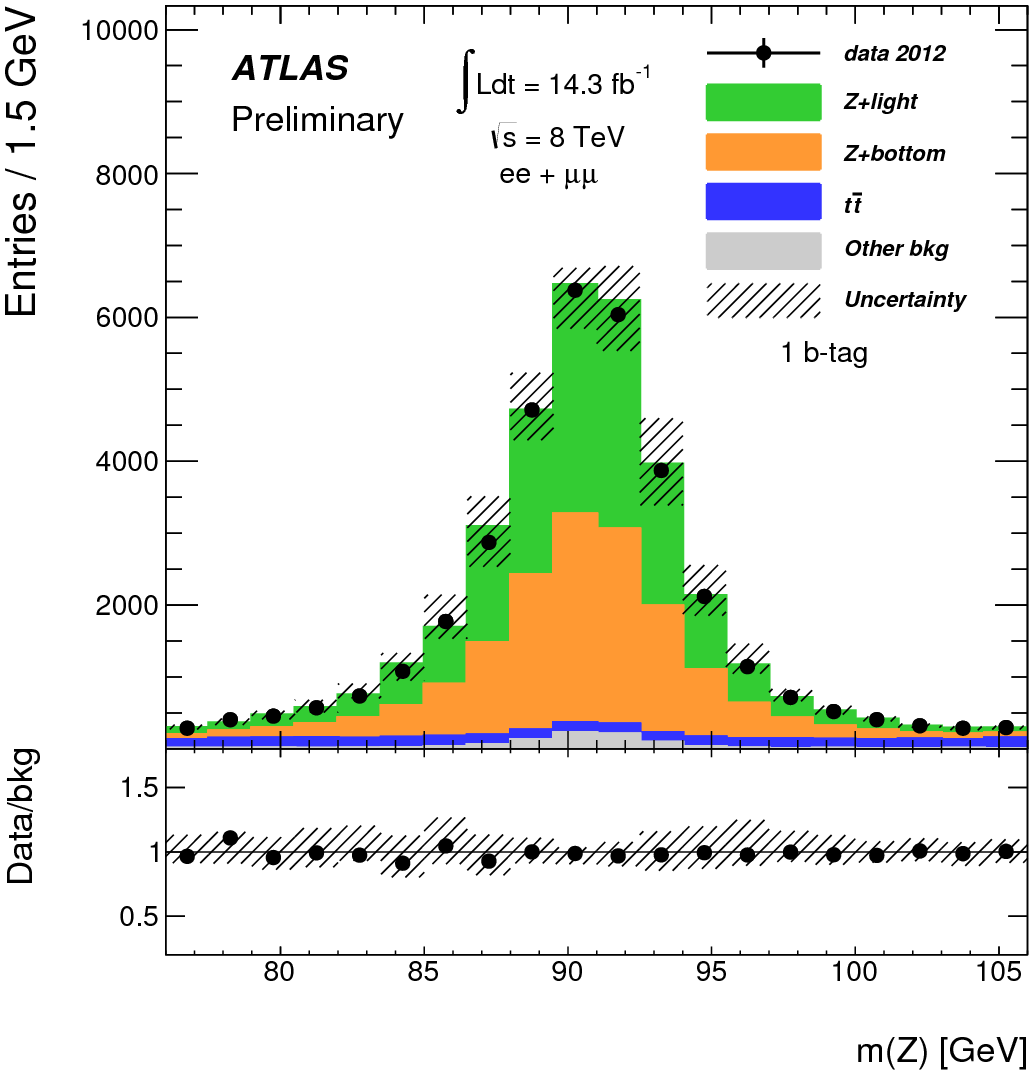
\includegraphics[width=.28\textwidth]{ztag/fig_04a}
       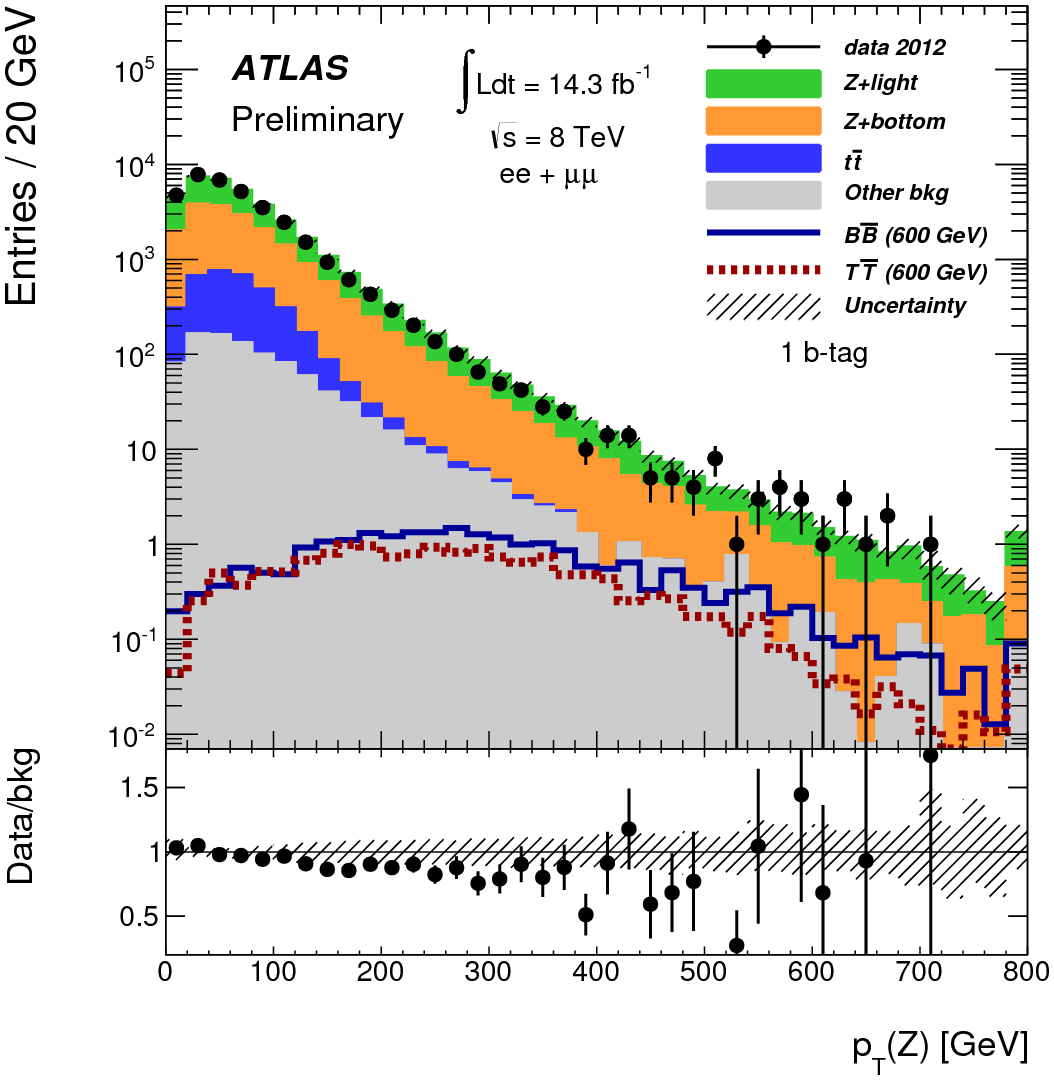
\includegraphics[width=.28\textwidth]{ztag/fig_05a}
       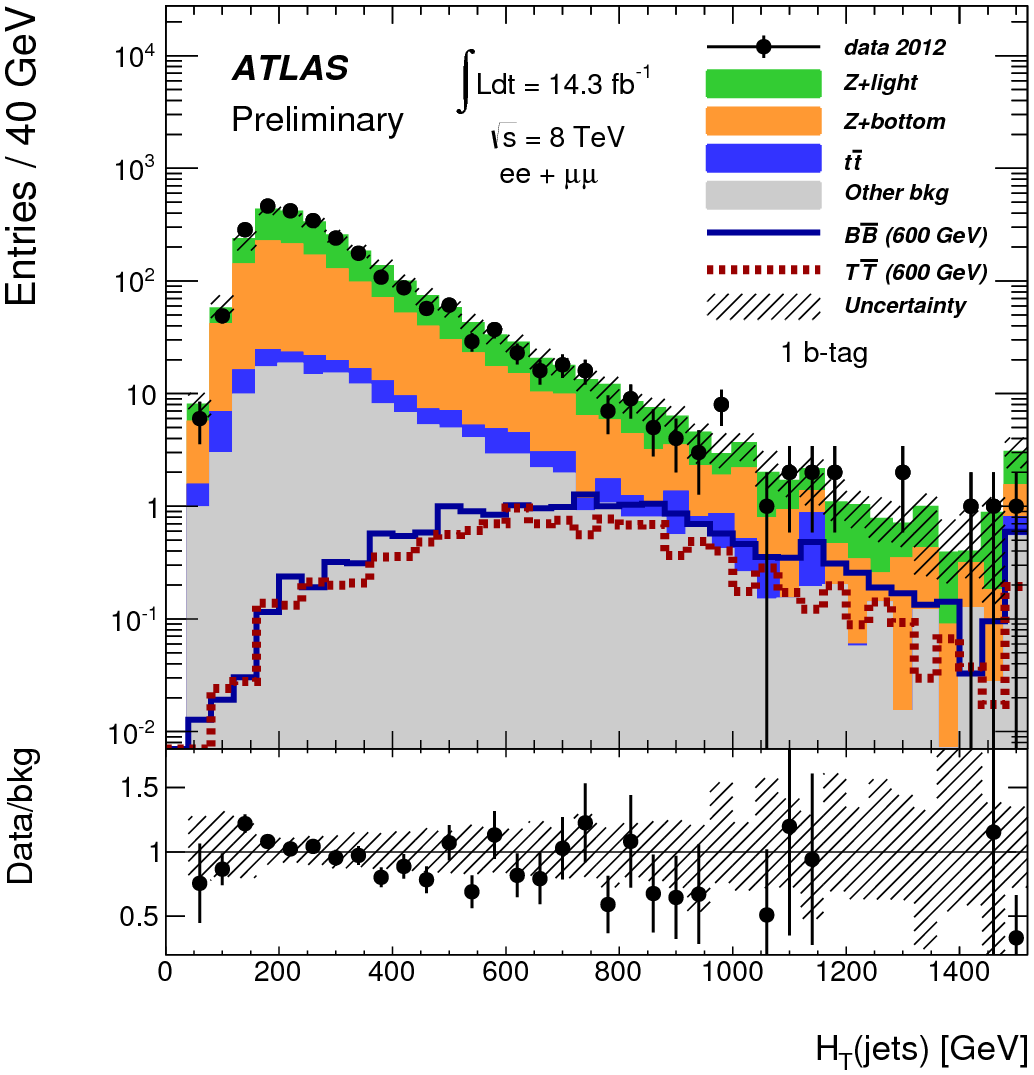
\includegraphics[width=.28\textwidth]{ztag/fig_06a}


       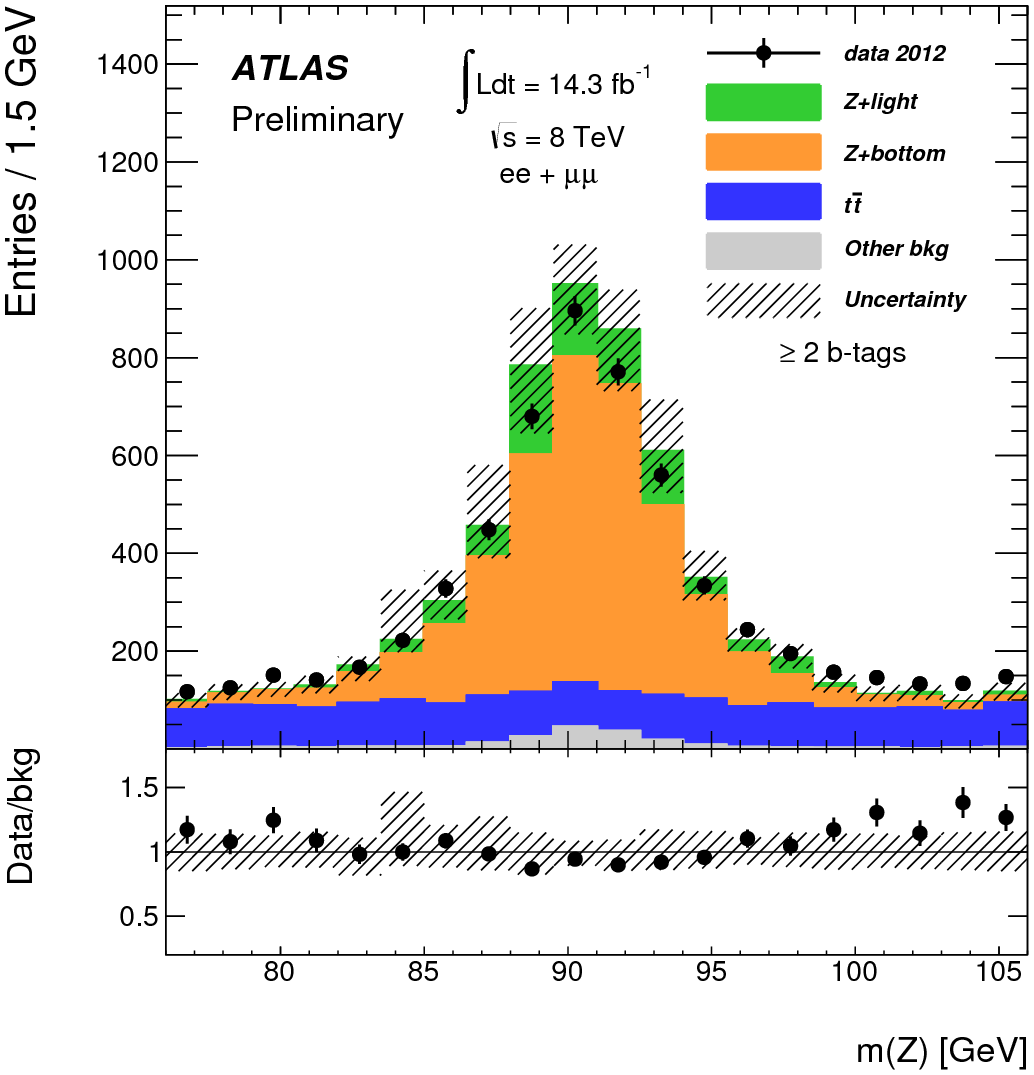
\includegraphics[width=.28\textwidth]{ztag/fig_04b}
       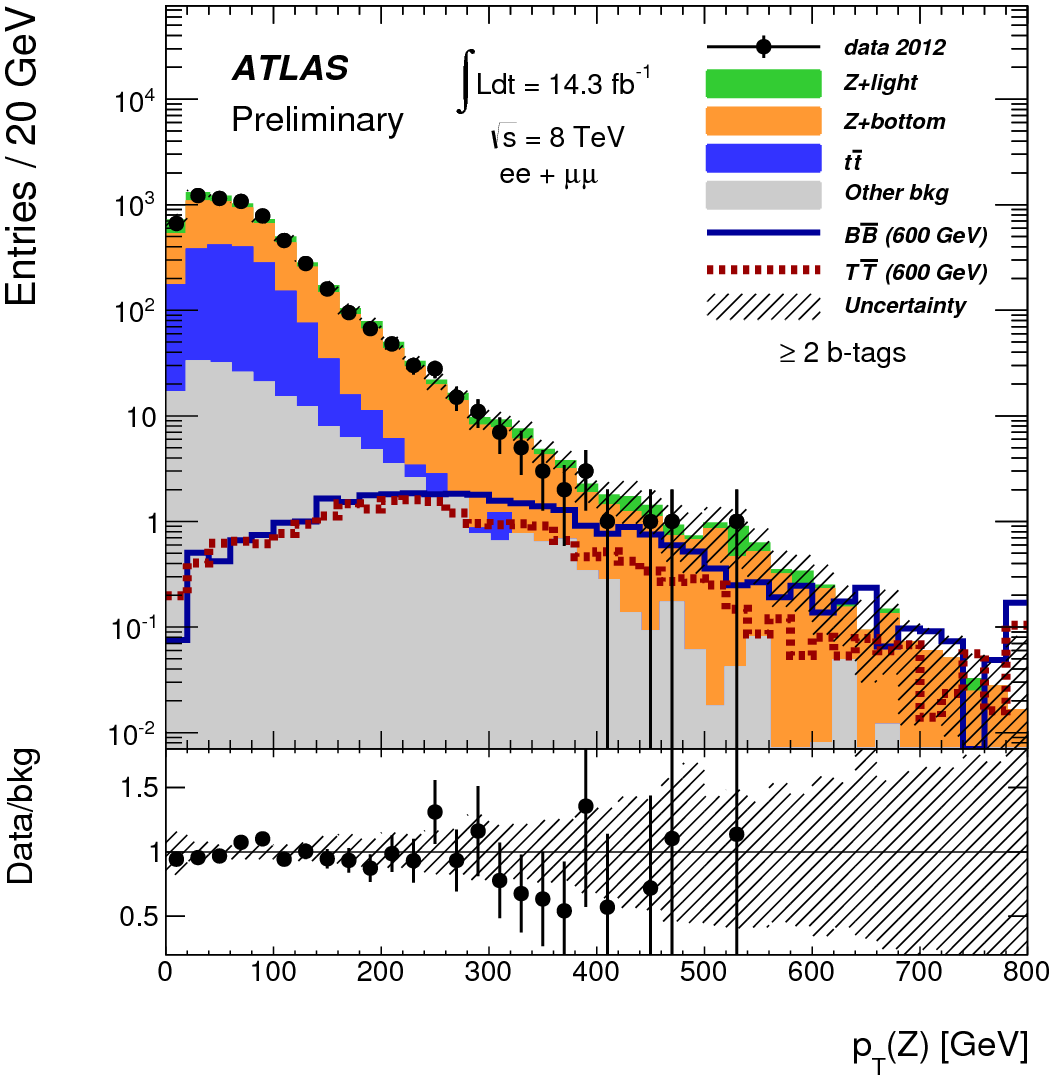
\includegraphics[width=.28\textwidth]{ztag/fig_05b}
       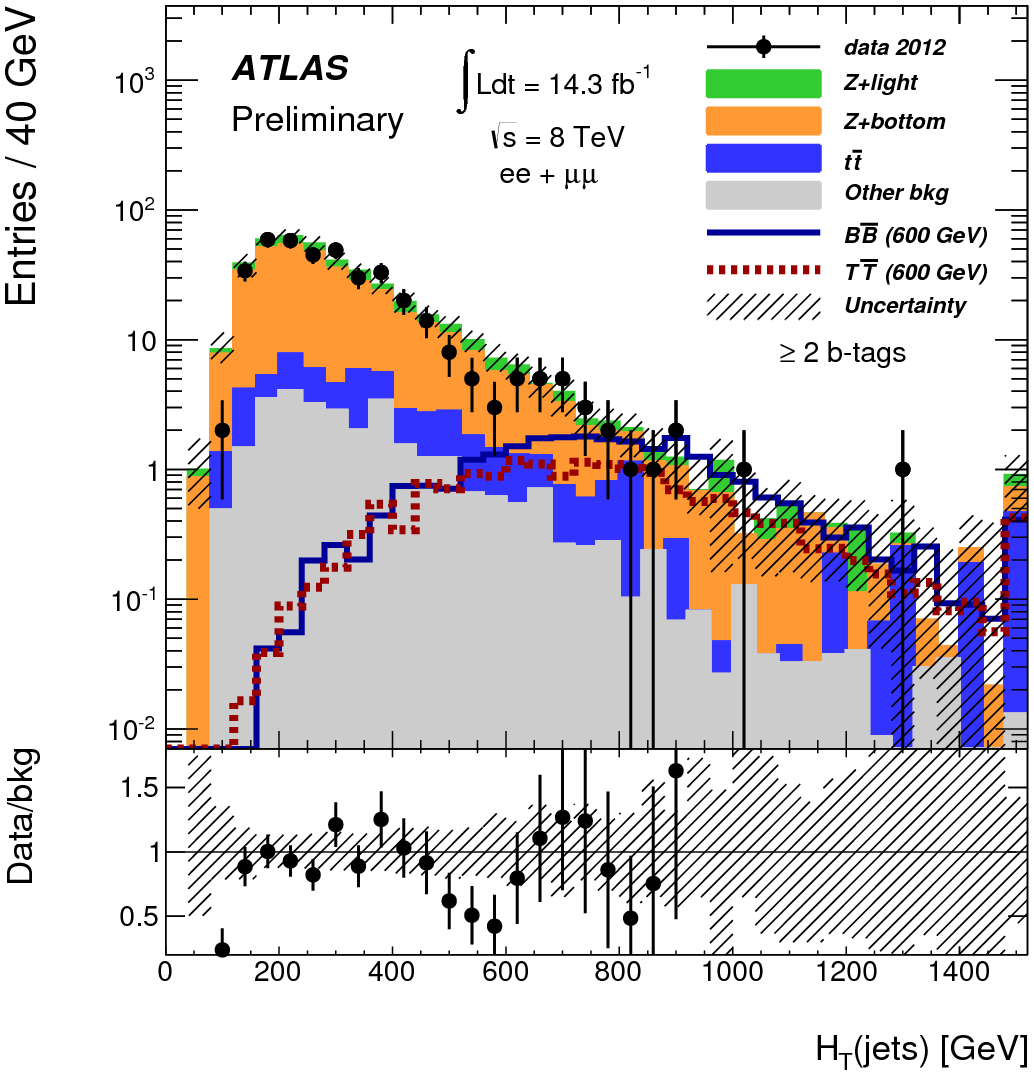
\includegraphics[width=.28\textwidth]{ztag/fig_06b}

\end{frame}

\begin{frame}\frametitle{$B\bar{B}(T\bar{T})\to Zb(t)+X$~\cite{ATLAS-CONF-2013-056}}
\footnotesize\centering

       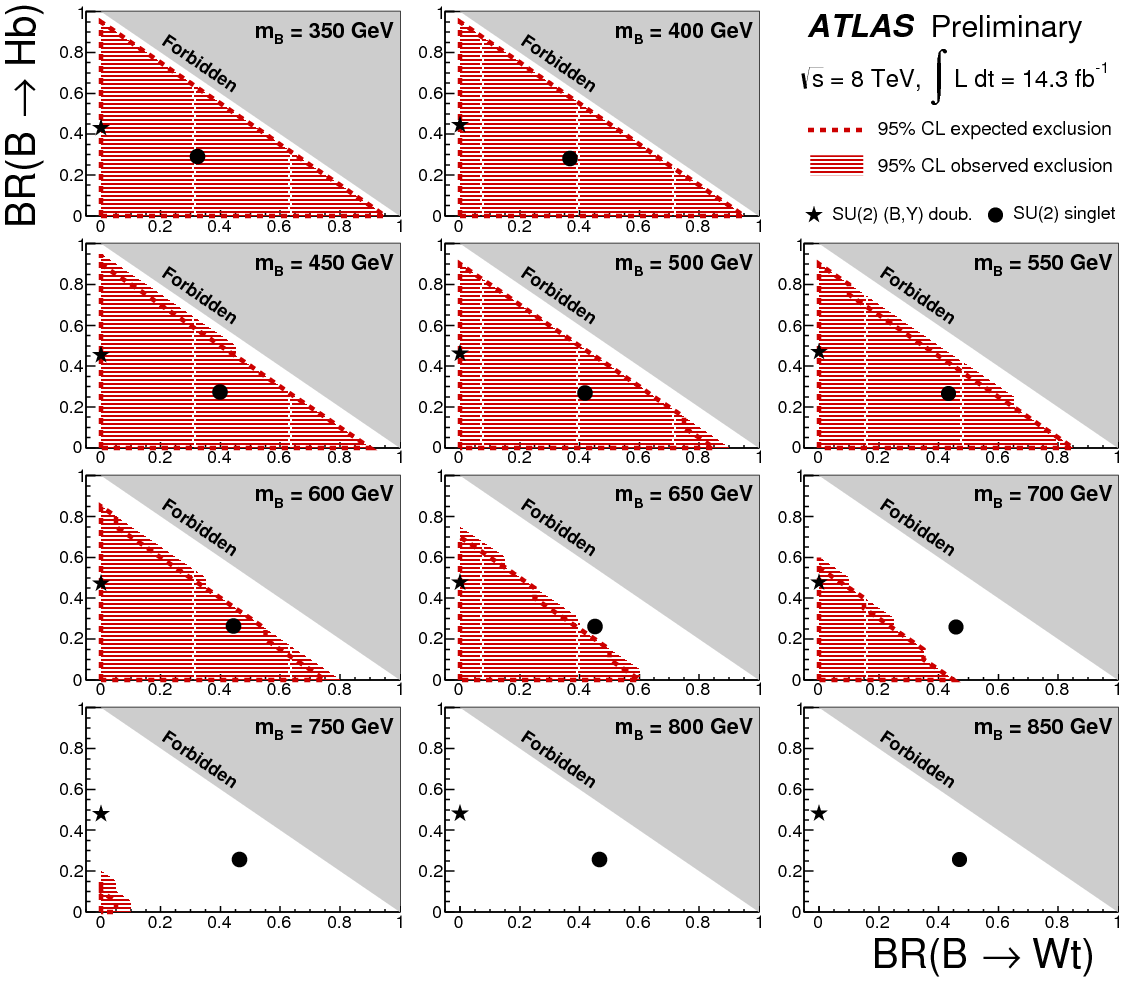
\includegraphics[width=.68\textwidth]{ztag/fig_10}

\end{frame}


\begin{frame}\frametitle{$B\bar{B}(T\bar{T})\to Zb(t)+X$~\cite{ATLAS-CONF-2013-056}}
\footnotesize\centering

       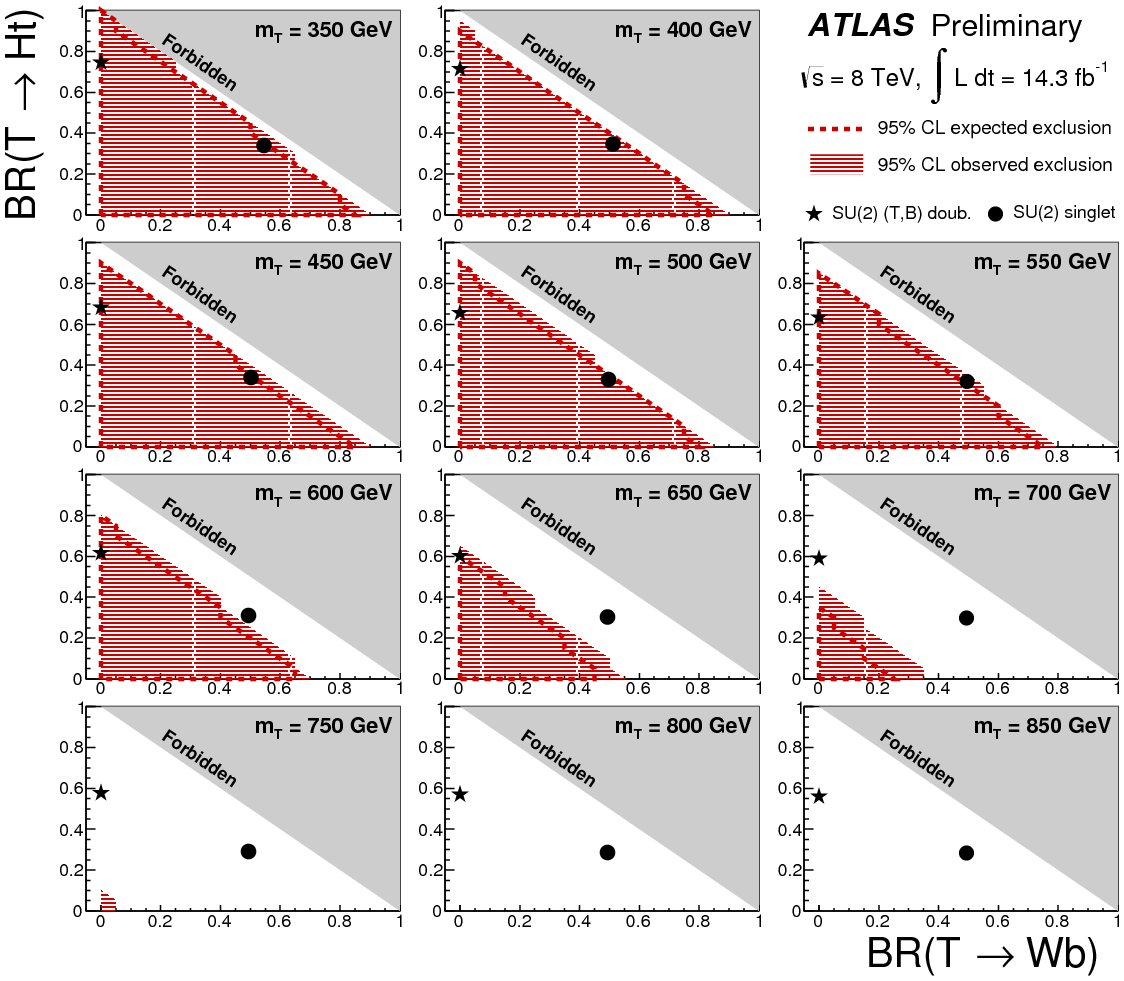
\includegraphics[width=.68\textwidth]{ztag/fig_11}

\end{frame}


\begin{frame}\frametitle{$B\bar{B}(T\bar{T})\to Zb(t)+X$~\cite{ATLAS-CONF-2013-056}}
\footnotesize\centering

       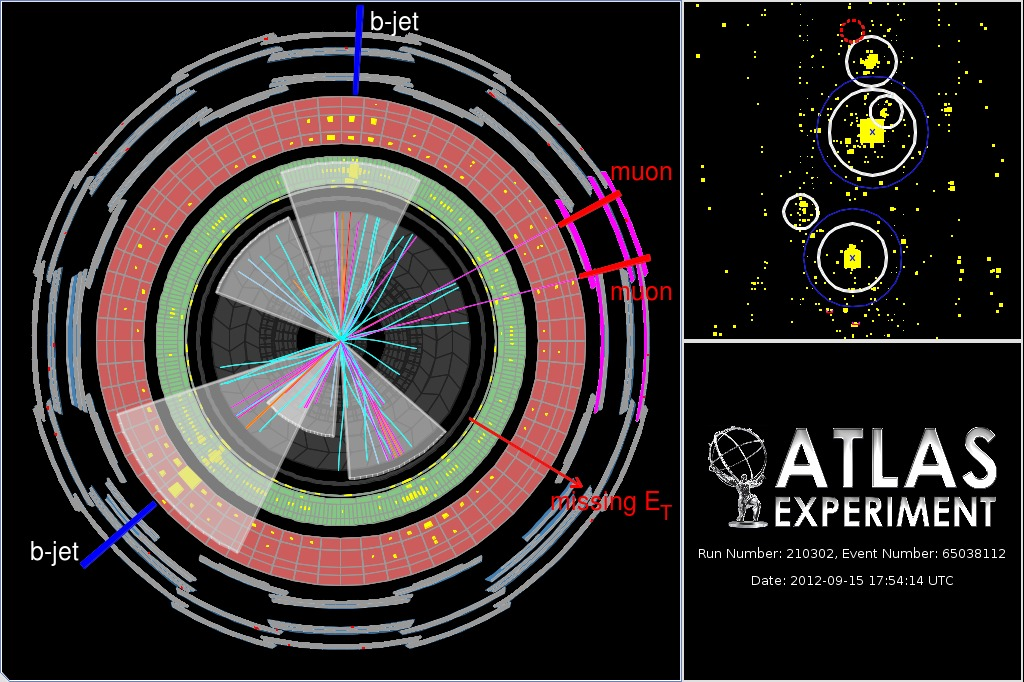
\includegraphics[width=.68\textwidth]{ztag/fig_14}

\end{frame}




\begin{frame}\frametitle{$T\bar{T}\to Wb+X$~\cite{ATLAS-CONF-2013-060}}
\scriptsize\centering

\begin{minipage}{.45\textwidth}\centering
    \begin{itemize}
    \item one lepton ($e$ or $mu$), ${E}^{\rm miss}_T >$20~GeV, ${E}^{\rm miss}_T + m_T(W)>$60~GeV
    \item $\geq$3 jets and one $W^{type I}_{had}$
    \end{itemize}
    OR 
    \begin{itemize}
    \item $\geq$4 jets and one $W^{type II}_{had}$ and no $W^{type I}_{had}$
    \item $\geq$ 1 $b$tagged jet (consider also the 2nd highest $b$-tag weight jet)
    \item $H_T^{(a)}>800~$GeV
    \item $p_T(b_1)>160~$GeV, $p_T(b_2)>80~$GeV
    \item $\Delta R(l,\nu) < 1.2$
    \item $min(\Delta R(l,b_{1,2})) > 1.4$
    \item $min(\Delta R(W_{had},b_{1,2})) > 1.4$
    \end{itemize}
\end{minipage}\begin{minipage}{.55\textwidth}\centering  

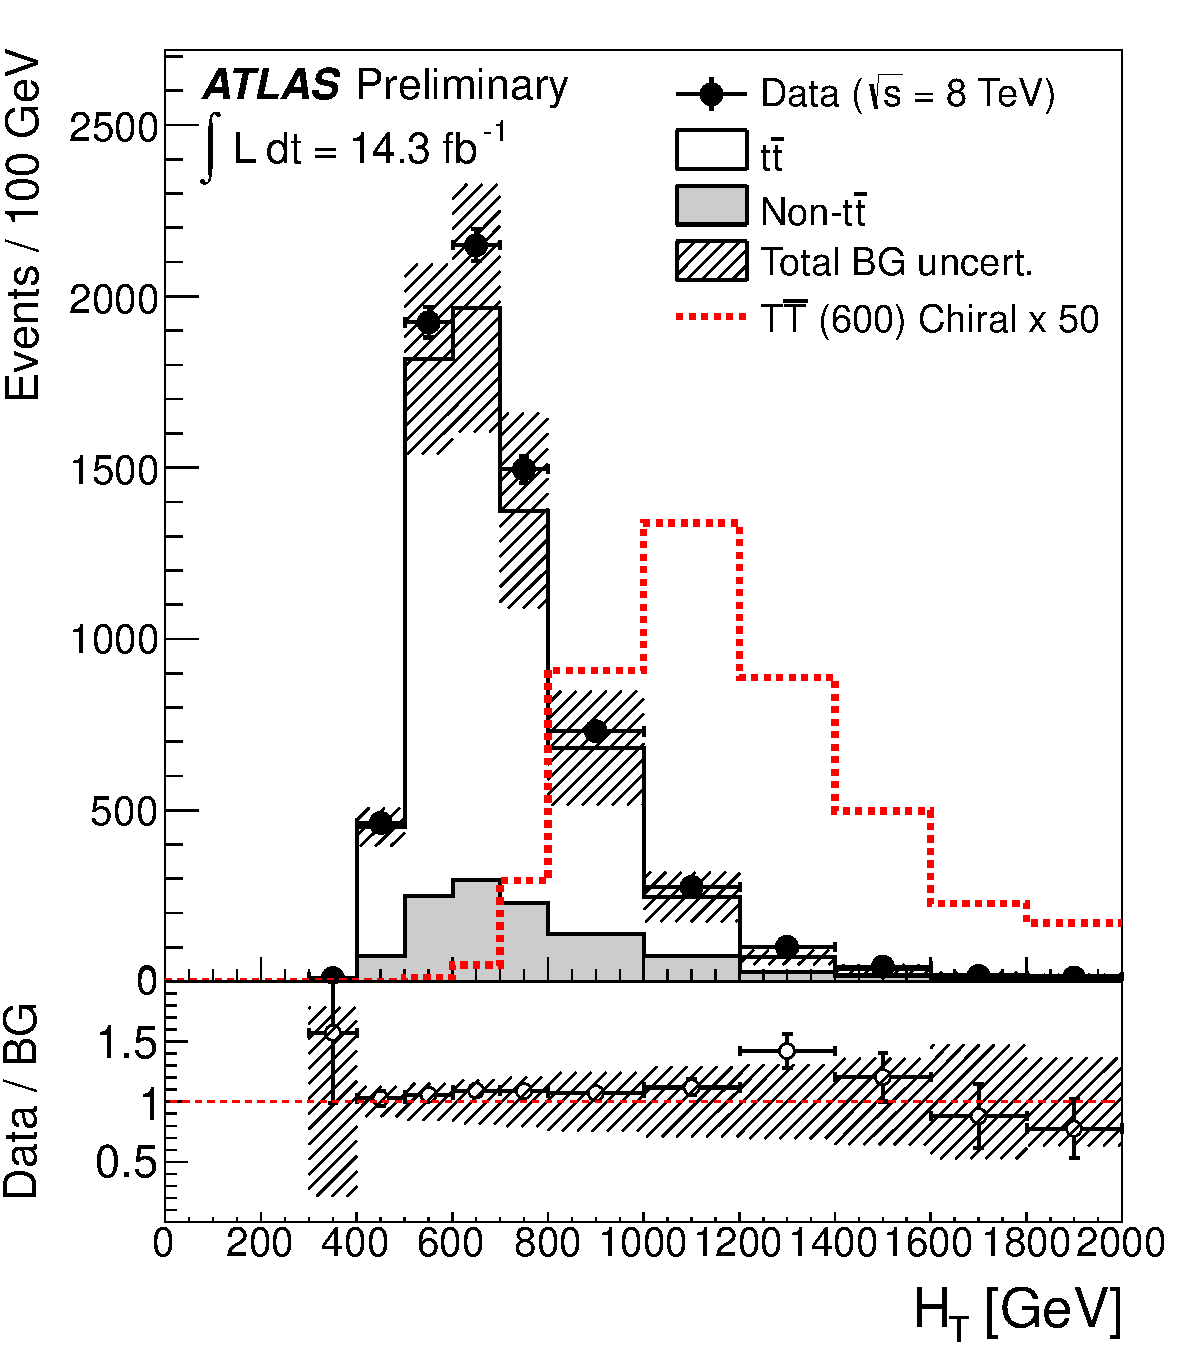
\includegraphics[width=.5\textwidth]{wbx/fig_03b}
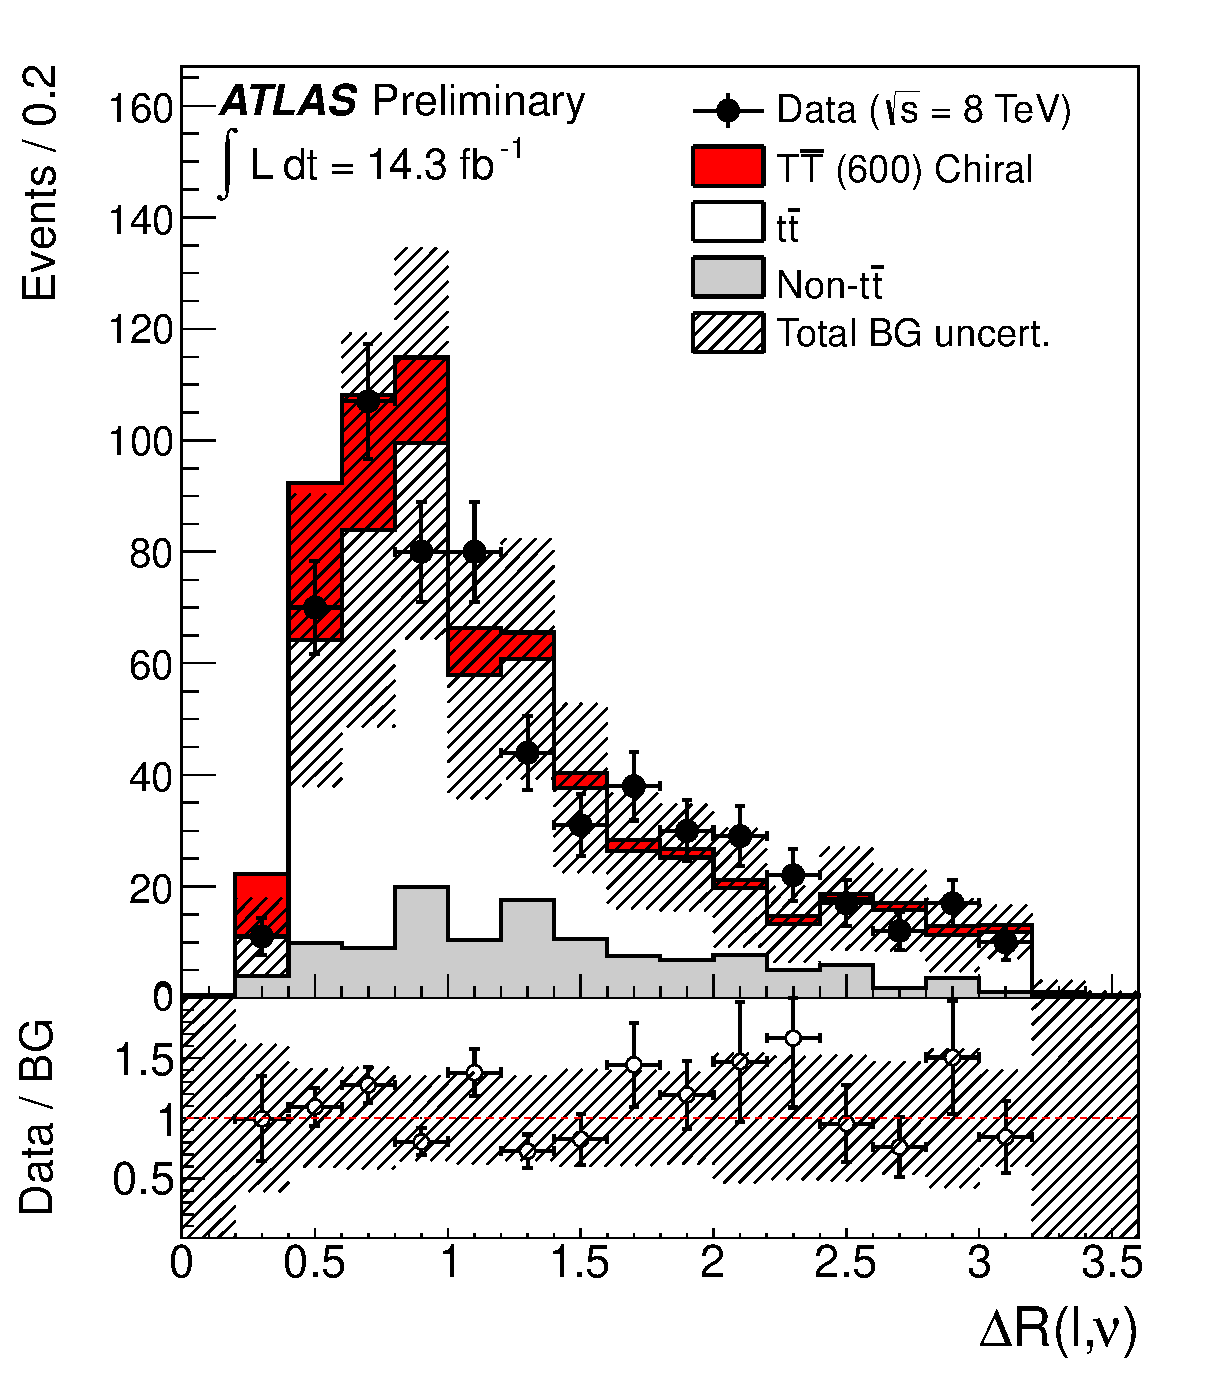
\includegraphics[width=.5\textwidth]{wbx/fig_05a}

\end{minipage}


\tiny $$^{(a)} H_T = p_T(j_1) + p_T(j_2) + p_T(j_3) + p_T(j_4) + p_T(l) + E_T^{\rm miss}$$
\end{frame}


\begin{frame}\frametitle{$T\bar{T}\to Wb+X$~\cite{ATLAS-CONF-2013-060}}
\footnotesize\centering

       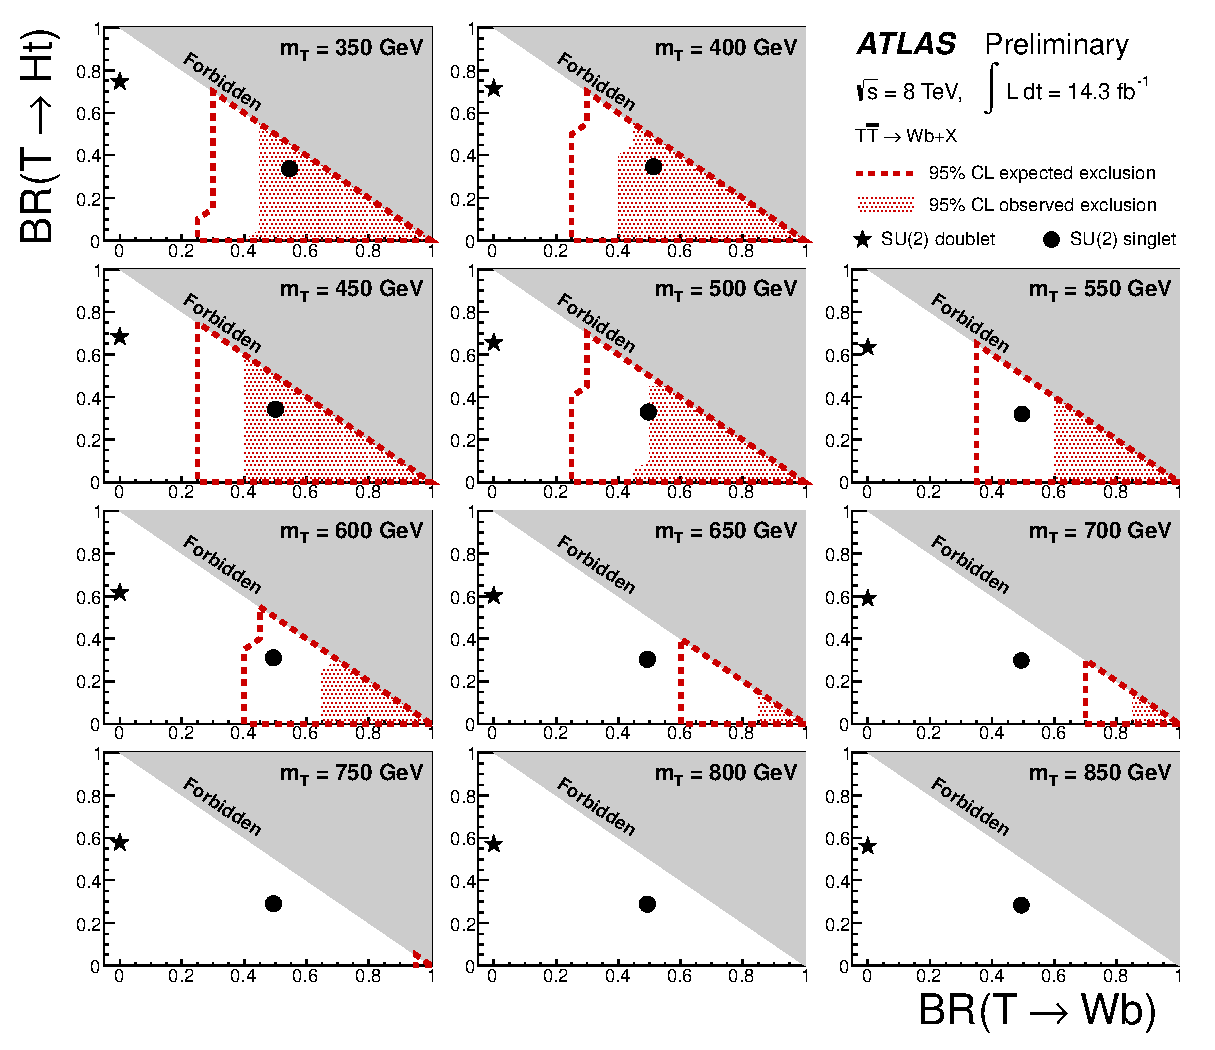
\includegraphics[width=.7\textwidth]{wbx/fig_08}

\end{frame}


\begin{frame}\frametitle{combining $T\bar{T}\to Ht+X$~\cite{ATLAS-CONF-2013-018} and $T\bar{T}\to Wb+X$~\cite{ATLAS-CONF-2013-060}}
\footnotesize\centering

       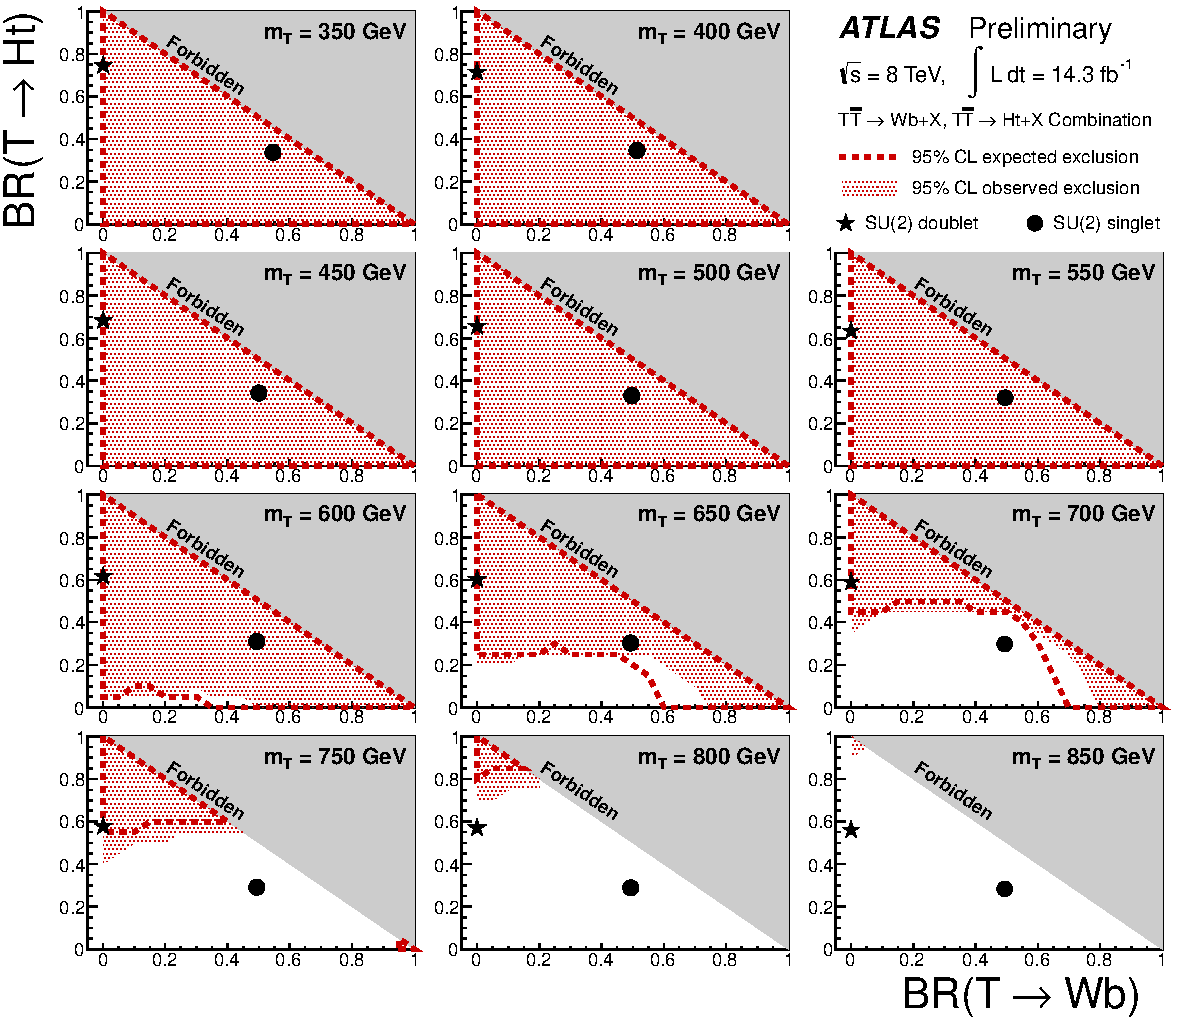
\includegraphics[width=.7\textwidth]{wbx/fig_10}

\end{frame}



\begin{frame}\frametitle{Results on chiral quarks: $b'\to Wt$ (100\%)~\cite{ATLAS-CONF-2013-051}}
\footnotesize\centering

       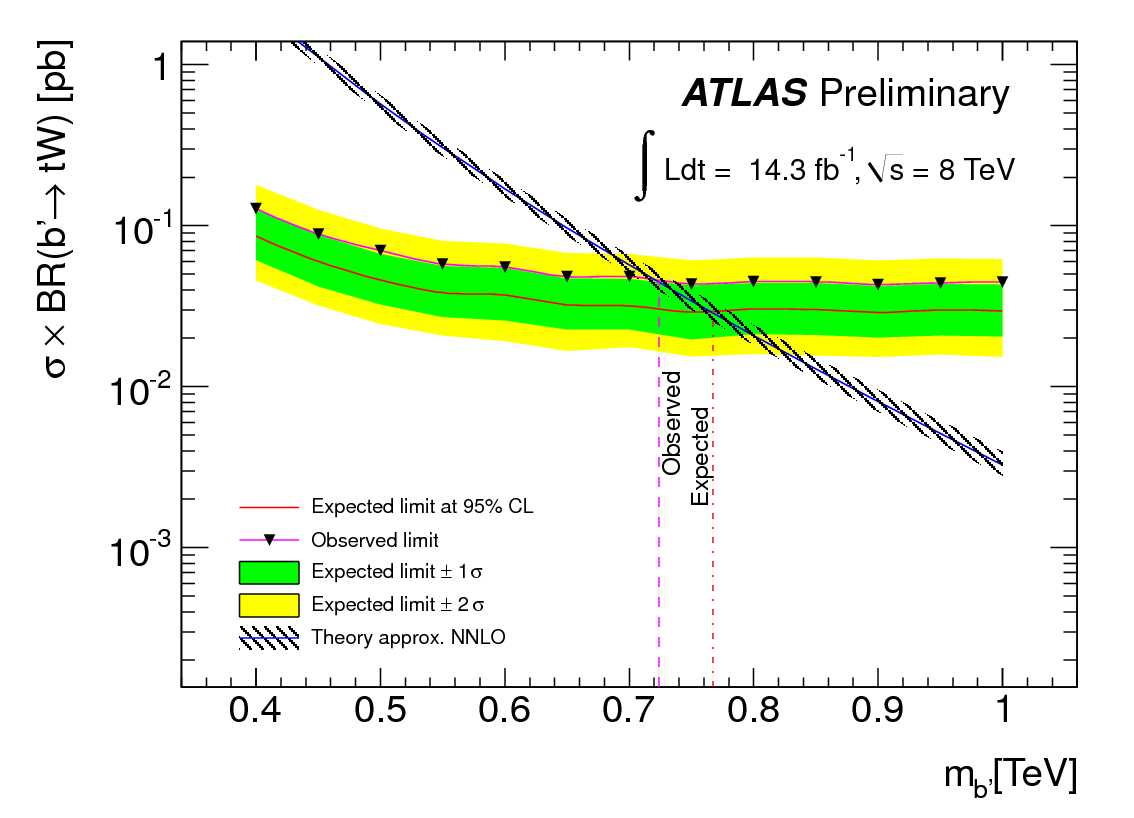
\includegraphics[width=.7\textwidth]{ssign/fig_04}

\end{frame}

\begin{frame}\frametitle{Results on chiral quarks: $t'\to Wb$ (100\%)~\cite{ATLAS-CONF-2013-060}}
\footnotesize\centering

       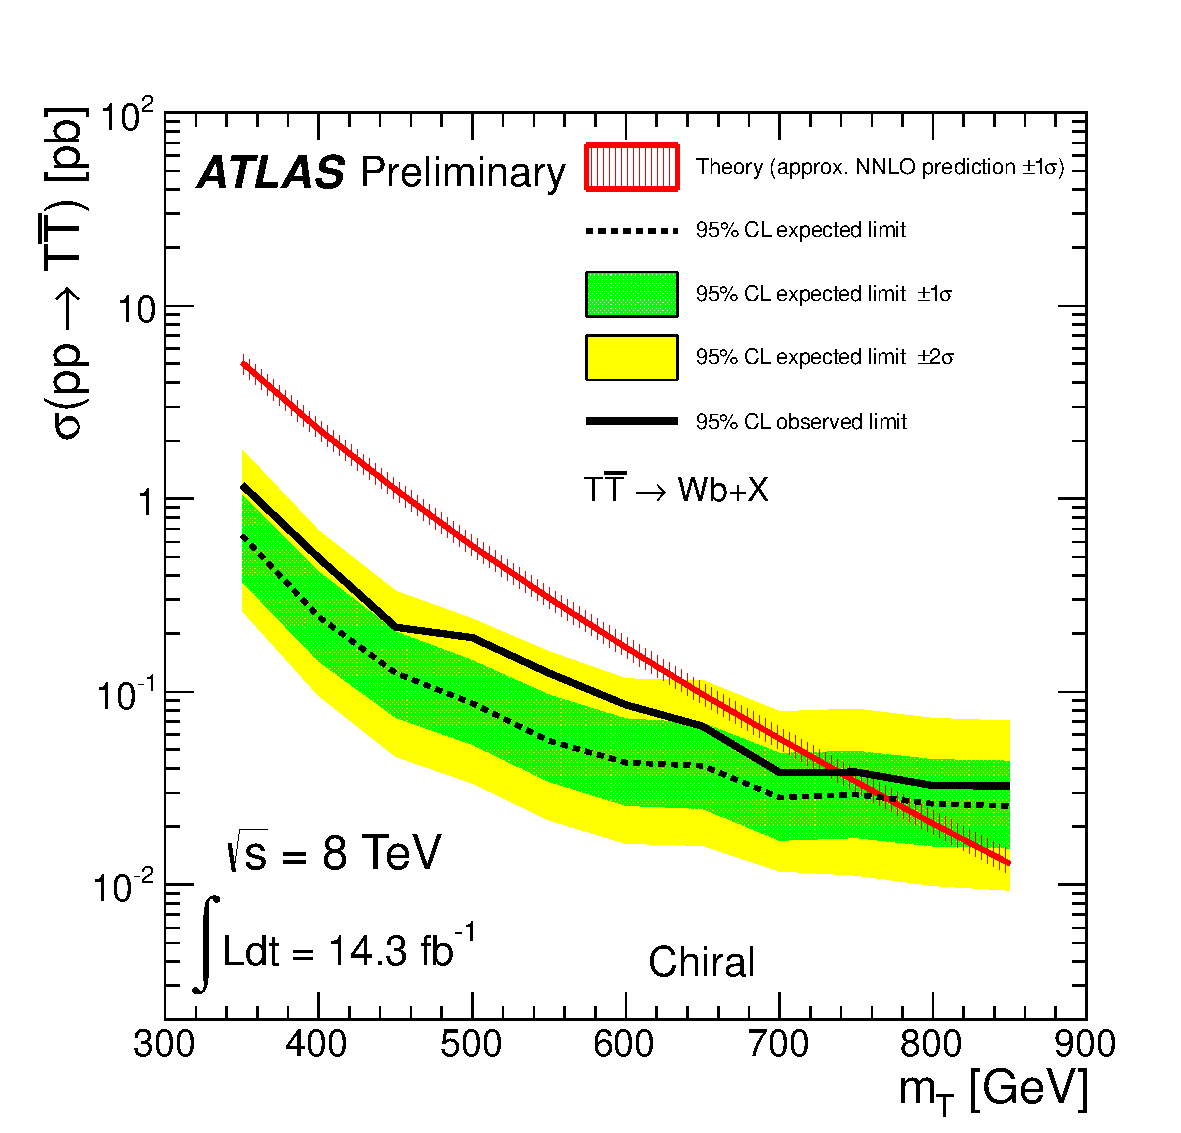
\includegraphics[width=.6\textwidth]{wbx/fig_07a}

\end{frame}





\BackgroundPicture{pics/atlas}

\begin{frame}\frametitle{The ATLAS Detector}
\footnotesize\centering

\footnotesize
\begin{minipage}{.35\textwidth}
A general purpose experiment
\begin{itemize}
\item vertex detector and central tracker
\item superconducting solenoid
\item electromagnetic and hadronic calorimeters
\item muon spectrometer
\item superconducting toroids
\item high hermeticity (full $\phi$ and $|\eta|<5$)
%\item fake electrons and photons rejection (rejection rate of 10$^5$ and 10$^3$)
%\item very selective and efficient trigger (rejection rate of 10$^7$)
\end{itemize}
%\vspace{1.5cm}
\end{minipage}\begin{minipage}{.6\textwidth}\centering\pause
\hspace{2cm}\begin{beamercolorbox}[wd=.9\textwidth,rounded=true,shadow=true]{whiteboxcolor}\centering
{\bfseries In 2012 21.7\ifb\  collected at $\sqrt{s}=8~$TeV!}
\vspace{.3cm}

\includegraphics[width=.8\textwidth]{pics/sumLumiByDay2012}

\vspace{\baselineskip}
%Reached peak luminosity of $3.65\times 10^{33}~$cm$^{-2}$s$^{-1}$\\
\end{beamercolorbox}

See \href{https://twiki.cern.ch/twiki/bin/view/AtlasPublic}{ATLAS public page}

\end{minipage}

\myskip
Will present results obtained with \alert{14.3\ifb}\ of 2012 data

\end{frame}


\BackgroundPicture{pics/emptyIMG}



\end{document}
